%%%为了方便排版采样Latex文件,由于目前查询到的版本在texlive环境下运行常出现错误,加以修正
%%%部分警告将完成修改后再进行上传
%%%目前版本已可以在texlive下顺利运行
\documentclass{Style/aas}
\usepackage{multicol}
\usepackage{subfigure}
\usepackage{amsmath}
\usepackage{amssymb}
\usepackage{amsfonts}
\usepackage{graphicx}
\usepackage{url}
\usepackage{ccaption}
\usepackage{booktabs} % 做三线表的上下两条粗线用

\setcounter{page}{1}

\begin{document}

\cntitle{{\hei\qquad 关于新颖异常检测的综述}

  \thanks{收稿日期\
    XXXX-XX-XX
    \quad
    录用日期\
    XXXX-XX-XX}

  \thanks{Manuscript received
    Month Date, Year;
    accepted
    Month Date, Year}

  \thanks{国家重点基础研究发展计划(973计划) (XXXXXX),国家高技术研究发展计划(863计划) (XXXXXX),国家自然科学基金(XXXXXX)资助}

  \thanks{Supported by National Basic Research Program of China (973 Program) (XXXXXX),
    National High Technology Research and Development Program of China (863 Program) (XXXXXX),
    National Natural Science Foundation of China (XXXXXX)}

  \thanks{本文责任编委\ XXX}

  \thanks{Recommended by Associate Editor BIAN Wei}

  \thanks{1.
    中国科学院自动化研究所高技术创新中心\ 北京\ 100190
    \quad 2.
    中国科学院自动化研究所模式识别国家重点实验室\ 北京\ 100190
    \quad 3.
    中国科学院自动化研究所《国际自动化与计算杂志》编辑部\ 北京\ 100190
    \quad 4. 中国科学院自动化研究所《自动化学报(英文版)》编辑部\ 北京\ 100190
    \quad 5. 中国科学院自动化研究所《自动化学报》编辑部\ 北京\ 100190}

  \thanks{1.
    Hi-Tech Innovation Center, Institute of Automation, Chinese Academy of Sciences, Beijing
    100190
    \quad 2.
    National Laboratory of Pattern Recognition,
    Institute of Automation, Chinese Academy of Sciences, Beijing 100190
    \quad 3.
    Editorial
    Office of {\sl International Journal of Automation and Computing},
    Institute of Automation, Chinese Academy of Sciences, Beijing 100190
    \quad 4. Editorial
    Office of {\sl IEEE/CAA Journal of Automatica Sinica (JAS)}, Institute of Automation,
    Chinese Academy of Sciences, Beijing 100190
    \quad 5. Editorial
    Office of {\sl Acta Automatica Sinica}, Institute of Automation,
    Chinese Academy of Sciences, Beijing 100190
  }}

\cnauthor{尚书林$^{\scriptscriptstyle1,\,2}$
  \hspace{1em}
  左年明$^{\scriptscriptstyle2}$
  \hspace{1em}
  陈培颖$^{\scriptscriptstyle3}$
  \hspace{1em}
  欧\ 彦$^{\scriptscriptstyle4,\,5}$
  \hspace{1em}
  张\ 哲$^{\scriptscriptstyle4,\,5}$
}

\cnabstract{近年来鲜有对新颖性检测领域进行完整严谨的综述,本文新颖地运用多层次分类方法,从方法适配数据层面对2017-2020年间的经典文献进行分析,对本领域的应用热点进行了深入探究,方便其他领域研究者在识别其领域新颖或“未知”内容时,有方法可循.本文介绍了新颖性检测的基本概念,区分了与其极易混淆的术语,并且在早期新颖性检测综述基础上增加了热门方法类别,这为今后的研究工作提供了有价值的依据和参考.本文独特分析角度,或许可以启发研究者以数据驱动的思想,把握分析各个数据领域新颖动向;同时不同数据类型上思想和方法上的碰撞,也可以帮助研究者们思考出应用更为广泛的新颖性检测算法.}

\cnkeyword{新颖性检测,多层次分类,数据类型,算法应用}

\doi{10.16383/j.aas.20xx.cxxxxxx}

\entitle{Preparation of Papers for Acta Automatica Sinica}

\enauthor{SHANG Shu-Lin$^{1,\,2}$
  \qquad
  ZUO Nian-Ming$^2$
  \qquad
  CHEN Pei-Ying$^3$
  \qquad
  OU Yan$^{4,\,5}$
  \qquad
  ZHANG Zhe$^{4,\,5}$
}

\enabstract{In recent years, there have been few complete and rigorous reviews in the field of novelty detection. This article creatively uses a multi-level classification method to review the classic journals from 2017 to 2020 from the perspective of data adaptation and conducts an in-depth exploration of the application hotspots in this field. In this way, it is convenient for researchers in other fields to have the method reference based on the novelty detection, and it can even enlighten researchers to analyze data trends in other fields driven by the data-oriented thinking when identifying the novelty or "unknown" contents about research. In the article, we also introduce the basic concepts of novelty detection, distinguishes different terms that are easily confused with it, and on the basis of the early novelty detection review, the category of popular methods has been added, which provides valuable reference and fountain for future research. The unique analytical perspective of this article may inspire researchers to use data-driven thinking to grasp and analyze new trends in various data fields; at the same time, different data types The collision between the above ideas and methods can also help researchers to think about more widely used novelty detection algorithms.}

\enkeyword{Novelty Detection,Multi-level Classification,Data Type}

\cnaddress{尚书林,左年明,陈培颖,欧彦,张哲.
  《自动化学报》稿件加工样本. 自动化学报, 201X,
  \textbf{XX}(X): X$-$X}

\enaddress{Shang Shu-Lin, Zuo Nian-Ming, Chen Pei-Ying, Ou Yan, Zhang Zhe.
  Preparation of papers for Acta Automatica Sinica.
  \textsl{Acta Automatica Sinica}, 201X, \textbf{XX}(X): X$-$X}

\maketitle

\pagestyle{aasheadings}

%这一章为引言,无需写标题.
在我们实际生活中, 尤其是在数据分析和决策任务中, 我们常常需要判断观察的数据项是否正常, 这在信用卡欺诈检测、患者疾病诊断、设备故障检测中很常见. 在这些情况中, 我们想知道何时可以将系统的行为判断为正常, 何时其又是异常的, 这之中最关键的问题在于: 在数据空间中区分正常项目和新颖项目(异常)的界限在哪里\cite{bartkowiak2011anomaly}.

而现代高完备系统的异常模式非常罕见, 甚至可能没有描述故障情况的数据2. “异常”示例的稀缺性可能是由于高昂的测量成本或发生异常事件的频率较低造成的. 例如, 医学诊断中可能有数百个测试结果, 但很少会显示特定疾病的症状;机器故障识别任务中其正常状态的测量价格便宜且易于获得, 而故障状态的测量将要求以所有可能的方式销毁类\onecolumn\begin{multicols}{2}似的机器. 因此, 即使不是不可能, 也很难获得很好采样的负类3. 另外, 异常定义模糊不清, 同时系统间的复杂性使得我们只能获得对各种系统组件间的有限理解. 由此产生的一个不可避免的结果是: 大量可能的“异常模式”中存在一些不是先验的异常, 在这种情况下, 我们只能使用正常类的信息来判断异常, 这使得传统的多分类方案不适合这些应用.

  鉴于我们永远无法在所有可能的对象类别上对系统进行训练, 因此在测试过程中能够区分已知对象信息和未知对象信息变得非常重要. 在实践中, 多项研究已经意识到, 新颖性检测是解决这一问题的最有效方法2.

  \section{基本概念}
  对于动物来说, 意外的感知可能是指潜在的掠食者或可能的受害者. 通过检测新的刺激, 其注意力首先会指向当前环境中最潜在的危险特征. 这种方式可以减少动物所接收的大量无关信息, 从而使其可以专注于异常刺激, 这便是自然界中动物的新颖性检测. 引申到人工学习系统中, 新颖性检测是指对新的或未知的数据或机器学习系统在训练期间未意识到的信号的识别4. 越来越多的领域专家表明这些新颖(未知)信号才是他们真正感兴趣的,就像分析人口变化时, 可能暗示着一个新的种类出现1.

  新颖性检测的概念是在单分类框架中提出的2, 通常应用于数据集中含有大量“正常”示例(正例), 并且没有足够数据来描述“异常”示例(影响示例)的情况, 其中“正常”示例必须与所有其他可能性区分开, 通常假设为“正常”示例的采样非常好,而其他类别采样严重不足. 在新颖性检测中, 关键的概念是对象之间的相似性1, 其通过构建一个模型, 用大量的实例来表示系统正常运作的数据, 然后将前所未见的模式与这部分正常模式进行比较来检测. 通常这样会得到某种形式的新颖性分数, 此时若设置一个阈值, 并设定超过此阈值的定义为异常, 此类异常便可以由此判断. 具体地, 推导一个正态性模型$ M\left( \theta \right) $, 其中, $\theta $表示模型的自由参数, 并用于计算新颖性得分$z\left( x \right) $, 并将其分配给以前未“见过”的测试数据$x$. 相对于正常模型有较大的新颖性分数$z\left( x \right) $, 则该模式对应于增加的“异常”, 即定义新颖性决策边界$z\left( x \right) =k$, 若$ z\left( x \right) \le k $, 则将$x$分类为“正常”;若$ z\left( x \right) >k $, 则将$x$分类为“异常”.

  \subsection{不同术语间差异}
  在文献中用Novelty Detection表示新颖性检测, 但多数文献常将Outlier Detection、Anomaly Detection与其混淆使用. 虽然, 三者都属于异常检测领域, 但它们还是存在根本差异的.

  Outlier Detection通常是指在没有数据先验知识的情况下确定异常值, 类似于无监督聚类的学习方法. 处理一组数据中的“Rogue”观察值(可能会对数据分析产生很大影响的观察值)的任务就属于Outlier Detection. 该任务假定离群点(outliers)会污染所使用的数据集, 目标是在模型构建阶段处理outliers的存在.

  Anomaly Detection通常需要数据被标记“正常”或“异常”, 类似于监督分类的学习方法. 通常对不符合预期模式或数据集中其他类别的观测值进行识别的任务属于Anomaly Detection. 该任务目标是在模型构建阶段对正常数据和异常数据都进行显式建模2.

  而Novelty Detection仅对正常态进行建模, 这种方法类似于半监督识别方法. 其目标是检测数据集中先前未观察到(新颖)的模式, 例如新闻中的新讨论话题. 新模式和异常之间的区别在于, 新模式通常在被检测后可以并入正常模型中5. 给定一个P维数据集, 其中的数据来自同一个分布, 此时提供一个新数据点, 判断这个新数据点是否也来自同一个分布, 这是Novelty Detection要做的工作. 通常Novelty Detection的思路是训练一个大致的边界, 划定初始给定数据集大致的分布范围, 当数据点落在边界范围内时, 则判断这一新数据点来自与初始数据集相同的分布;若在边界范围之外, 就认为其不同于初始数据集的分布.

  Outlier Detection与Novelty Detection相似的地方在于它们的目标都是从常规观测值中区分异常值的, 但其区别主要体现在训练集数据中:Outlier Detection通常指训练数据中包含异常值, 且这些异常值被定义为远离其他观测值, 因此其会尝试在训练数据最集中的区域上进行拟合, 而忽略那些异常观测值, 这里的异常观测值通常也被称为“离群点、孤立点”;而Novelty Detection通常指训练数据不受异常值污染, 并且我们有兴趣去分析新观测值是不是异常值, 这里的异常值通常也被称为“新颖点”6.

  Anomaly Detection与Novelty Detection的区别是Anomaly Detection中的正常数据概念通常与Novelty Detection中所使用的概念不同. Anomalies通常被认为是“正常”数据中的不规则或瞬态事件, 这些事件通常是嘈杂事件, 会引起伪影, 而这些伪影会成为数据分析的障碍, 需要在执行分析之前将其删除. 根据这个定义可以知道新颖的数据不一定是Anomalies.

\end{multicols}

\begin{center}
  \vbox{\centering{\small 表1\quad 不同术语间差异
      \\
      Table 1 \quad The Differences Among Outlier Detection、Anomaly Detection and Novelty Detection} \vskip2mm
    \renewcommand{\baselinestretch}{1.2}
    {\footnotesize\centerline{\tabcolsep=15pt\begin{tabular*}{\textwidth}{ccp{160pt}c}
          \toprule
          术语                  & 任务类型 & 异常数据概念 & 对待异常值处理方式  \\
          \hline
          Outlier Detection     &  无监督     &     远离其他观测值的值(也被称为离群点、孤立点)       &      忽略该异常观测值       \\
          Anomaly Detection     &  有监督     &      “正常”数据中的不规则或瞬态事件(通常是嘈杂、会引起伪影事件)       &     在执行分析前需将其删除      \\
          Novelty Detection     &   半监督     &      不影响训练数据的值(也被称为新颖点、兴趣点)     &       通常在检测后将新模式并入正常模型中       \\
          \bottomrule
        \end{tabular*}}}}
\end{center}

\begin{multicols}{2}
  \subsection{本文分类准则}
  由于在机器学习领域内, 研究人员几乎都以数据类型为先划分研究方向, 因此, 本文以数据类型来归类总结新颖性检测, 这可以让其它领域内的研究人员更加便捷地定位到其领域中的新颖性检测方法. 而今生活中, 数据以文本、图形、图像、音频、视频等非结构化数据为主, 其相关数据急剧增加, 研究也日益热烈. 因此, 本次综述大致按照数据类型分类为图像数据(Image Data)、文本数据(Textual Data)、时序数据(Time-seriesData)以及其他数据四大类进行调查. 其中, 图片类、图形类、视频类等归为图像数据;办公文档、文字类等归为文本数据;时间序列类、音频类等归为时序数据;结构化数据、离散类、流数据类等归类为其他数据. 另外, 由于社交媒体数据多有文本及图片等两种以上数据类型, 因此也将其归为其他数据.

  为了能够有质量且完整地展现新颖性检测领域的研究现状, 本文选用了SCI、SSCI数据库中的文献资料进行分析, 通过关键词“Novelty Detection”, 时间跨度为2017-2020, 进行精确检索. 为了保证分析结果的有效性, 我们对获得的论文进行了有效的人工筛选, 筛选标题及关键词部分带有“Novelty Detection”的文章, 同时筛去内容重复或内容不相关的论文. 最终共获得国内外研究文献128篇, 作为本文的分析数据.
  \begin{center} {\centering
      \vbox{
        \centerline{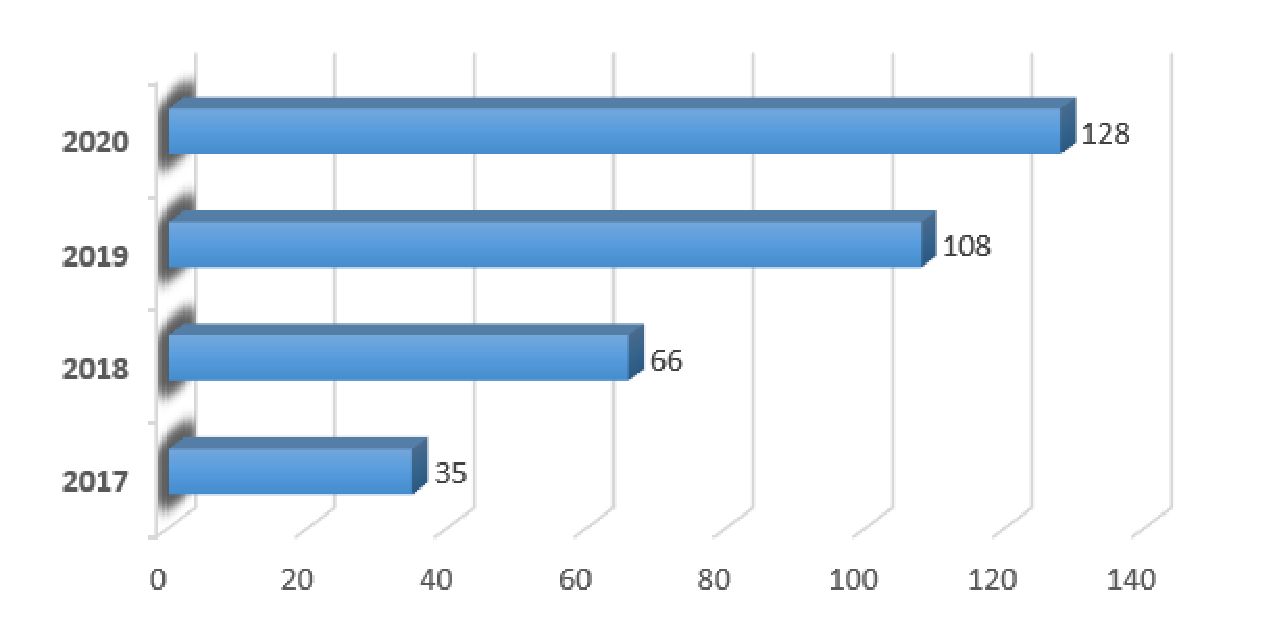
\includegraphics[width=8cm]{Image/counts.eps}}
        \vskip 1mm{\small
            图1\quad  2017-2020间新颖性检测领域发表文章累计量
            \\
            Fig.\,1\quad Yearly and Cumulative Count of Published Journals Related to Novelty Detection During 2017-2020 }
      }
    }
  \end{center}

  \begin{center} {\centering
      \vbox{

        \centerline{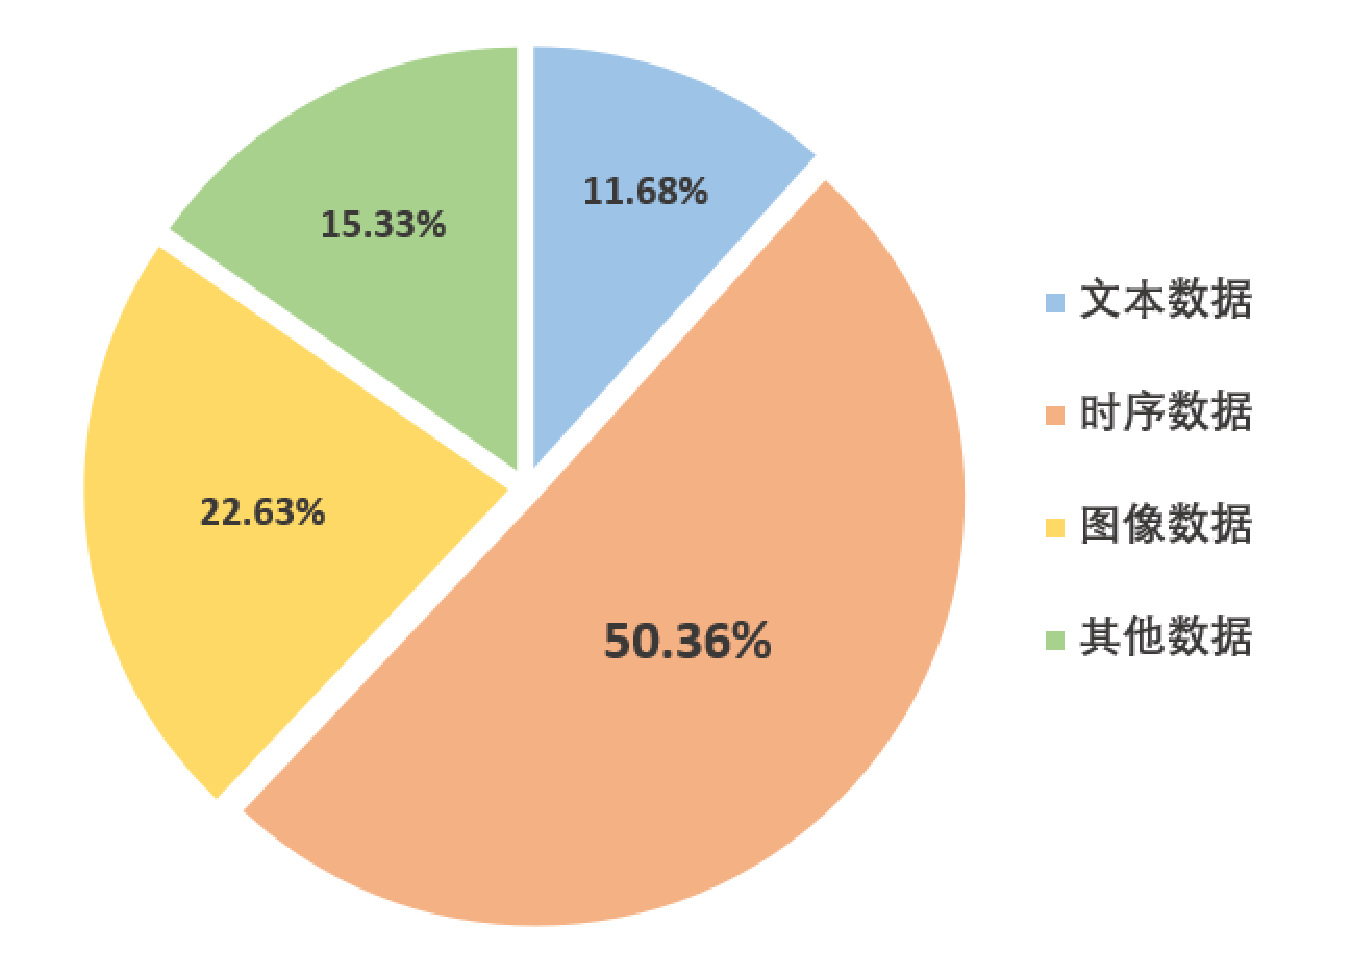
\includegraphics[width=5.5cm]{Image/rate.eps}}
        \vskip 1mm{\small
            图2\quad  2017-2020年有效数据类型占比
            \\
            Fig.\,2\quad The Proportion of Each Data Type During 2017-2020 }
      }
    }
  \end{center}


  \subsection{本文的组织结构}

  本综述介绍了新颖性检测的基本概念并区分了与其极易混淆的术语. 在本文的第二节, 介绍了新颖性检测领域方法类型. 在本文的第三节、第四节、第五节以及第六节, 分类介绍了时序数据、图像数据、文本数据以及其它数据类别下的新颖性检测算法应用. 在本文的第七节对本领域研究进行了总结.


  \section{新颖性检测方法}
  \begin{center} {\centering
      \vbox{

        \centerline{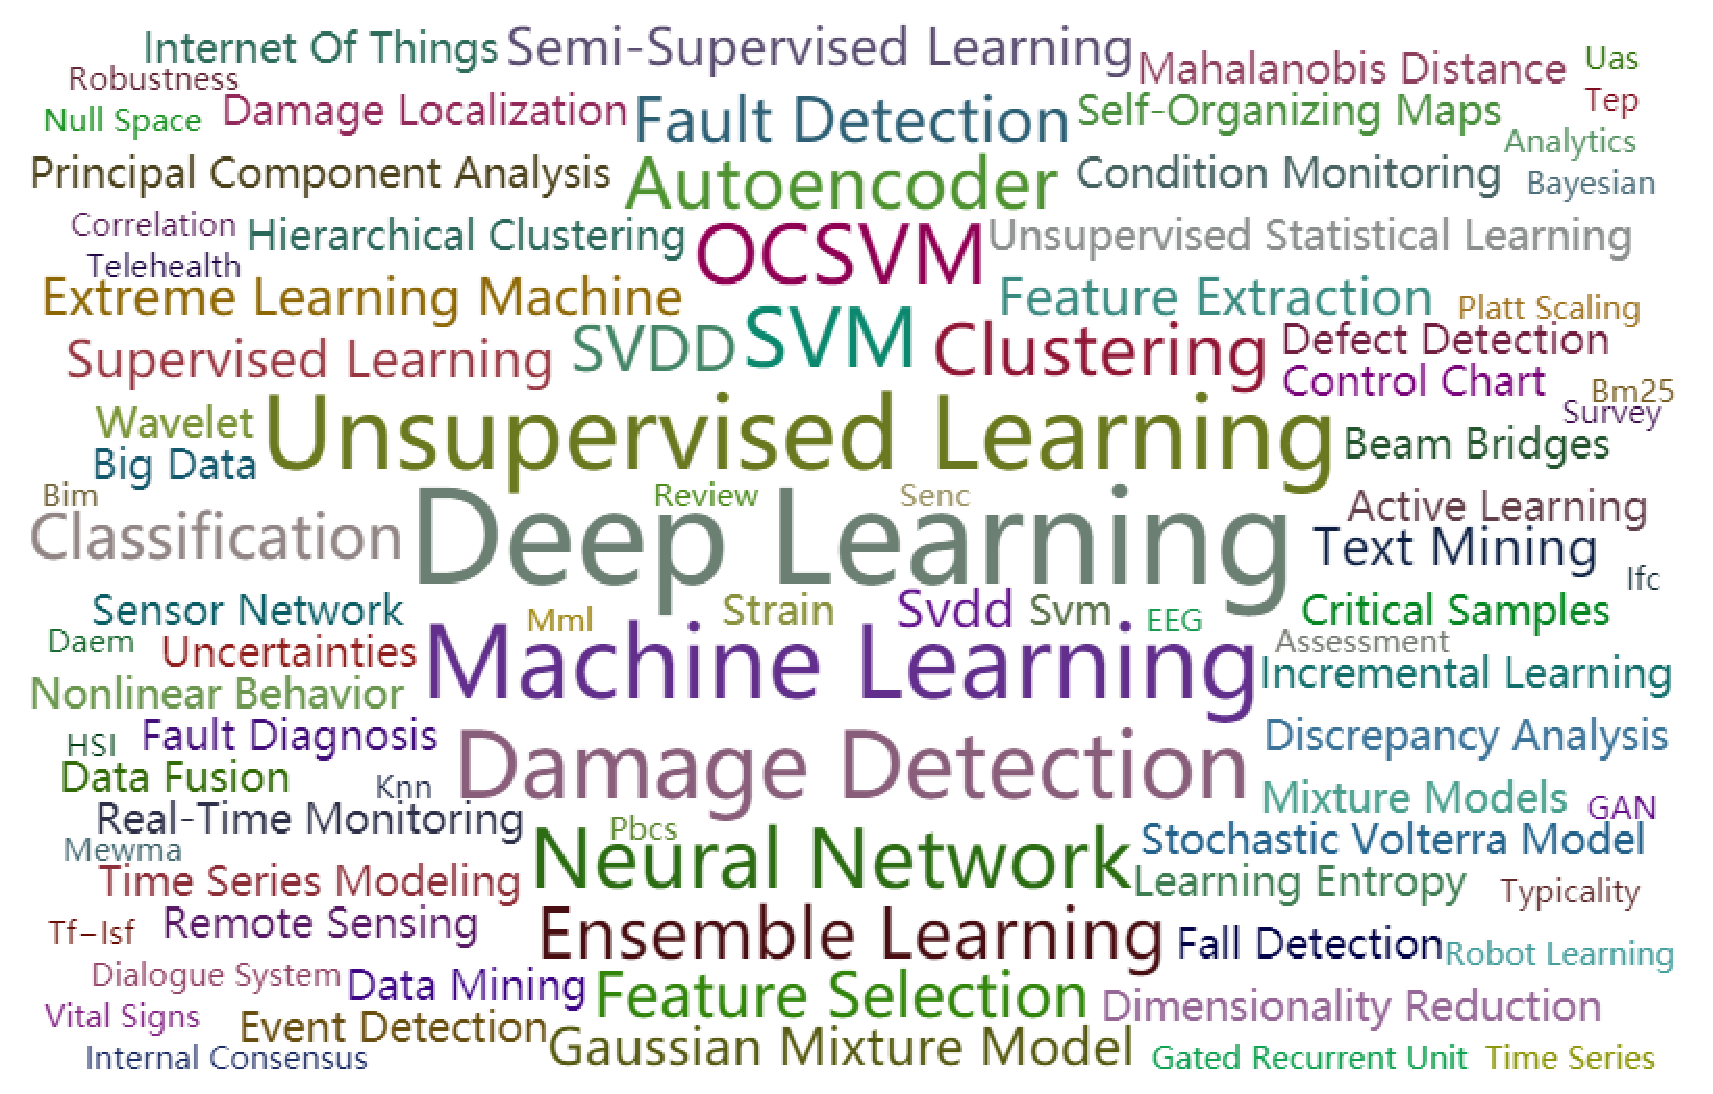
\includegraphics[width=8cm]{Image/wordcloud.eps}}
        \vskip 1mm{\small
            图3\quad  2017-2020文献关键词词云统计
            \\
            Fig.\,3\quad The Word Cloud Statistics for Keywords of Journals During 2017-2020 }
      }
    }
  \end{center}

  过去的新颖性检测算法从算法角度分类,通常可以分为五类:基于概率的方法,基于距离的方法,基于重构的方法,基于域的方法以及基于信息的方法。为了展现新颖性检测领域的研究现状, 本综述将统计的128篇新颖性检测文献关键词作以统计,如图3所示。可以看到深度学习与集成学习近年来在新颖性检测领域被广泛使用.

  \subsection{基于概率的方法}
  基于概率的方法,通常在训练集上估计概率密度函数,再根据密度估计来判定新颖性。该类方法中的概率密度函数描述了正常样本的空间分布情况, 认为高概率密度区域包含“正常”对象的可能性很大;低概率密度区域包含“正常”对象的可能性很小,更有可能是新颖数据。基于概率的方法通常可以划分为参数化方法与非参数化方法。

  参数化方法假设正常数据是由参数$\theta$和概率密度函数$P\left( \theta \right) $的基本参数分布生成的,其中参数$\theta$由给定的训练数据生成.连续变量最常用的分布形式为高斯分布, 其参数使用最大似然估计(MLE)估计, 对于高斯分布存在闭合形式解析解.参数化方法的典型示例是混合高斯模型(GMM)[13]和隐马尔科夫模型(HMM).混合高斯模型通常用于分析分布形式较为复杂的数据集,其通过训练集来估计正常类概率密度,参数可以使用最大似然估计或贝叶斯方法来估计. 该方法的局限在于混合模型需要大量的训练样例来估计模型参数, 所选择的数据分布函数形式也很可能不是拟合数据分布的良好模型.隐马尔科夫模型通常用于分析时间序列数据集,其假设存在潜在的隐藏状态产生观测值,并且这个状态会随着时间的推移而发生变化. 模型中隐状态间的转换受随机过程控制, 可观测事件的“发射”概率由一组与每个状态相关的概率分布所决定.

  非参数化方法无需假设模型的结构是固定的, 模型会随着样本个数的增加而变得复杂. 最简单的非参数化方法是使用直方图,通过定义一个新测试数据与基于直方图的正常状态间距离度量以确定其是否异常. 非参数化方法的典型示例是核密度估计器(KDE)[14] ,其通常使用分布在数据空间上的大量核来估计概率密度函数.核密度估计器通常采用Parzen窗方法[15],在每个数据点上放置一个核(通常是高斯核),并对来自每个核的局部贡献求和,其中各高斯核心以每个训练样本为中心并具有相同方差.

  ([13] Reynolds D A. Gaussian mixture models.[J]. Encyclopedia of biometrics, 2009, 741: 659-663.
  [14] Bishop C M. Pattern recognition and machine learning[M]. springer, 2006.)
  [15] Janakiram D, Kumar A, et al. Outlier detection in wireless sensor networks using Bayesian belief networks[C])

  \subsection{基于距离的方法}
  基于距离的新颖性检测方法,通过度量测试样本与训练样本间的距离来确定其是否为新颖数据。该方法通常基于最近邻和聚类分析的概念,并假定“正常”数据将紧密聚集在一起,而新颖数据则发生在离它们最近邻很远的位置。通常包括近邻法、密度法、聚类法等。

  近邻法通常假设正常数据点必须在“正常”训练集近邻位置,而测试集中新颖点远离那些训练集中的正常数据点。近邻法的关键是距离度量,常用的距离度量有欧氏距离、马氏距离等,其中欧式距离是单变量与多变量连续属性的流行选择.近邻法的典型示例为k-最近邻(KNN),其考虑到第k个最近邻的距离和考虑到k近邻的平均距离.

  密度法通常基于点周围局部密度与其邻居的局部密度之比,与基于概率的方法不同,此类方法是基于距离度量计算出来的. 其典型示例为局部异常因子(LOF) [18],其样本邻域的大小由包含用户提供的最小点数的区域所决定.

  聚类法通常假设“正常”类在数据空间中有少量的原型点, 通常使用从测试点到最近原型的最小距离来量化异常.该类别的典型示例为K 平均算法(K-means) [17],通过选择k个随机初始聚类中心,并根据计算这些聚类中心与训练集中每个点间的距离更新当前聚类中心,直至不再更新时停止迭代。

  ([16] Peterson L E. K-nearest neighbor[J]. Scholarpedia, 2009, 4(2): 1883.
  [17] Lee H j, Roberts S J. On-line novelty detection using the kalman filter and extreme value
  theory[C]
    [18] Breunig M M, Kriegel H P, Ng R T, et al. Lof: identifying density-based local outliers[C])

  \subsection{基于重构的方法}
  基于重构的新颖性检测方法,通常使用训练回归模型来映射“新颖”数据,基于回归目标与实际观测值之间的重构误差来定义新颖性。该类别下的常用流程为将数据投影或嵌入到较低维空间中,并在该维空间中的少量特征用于描述正常样本,再通过测试样本与训练模型参数间的相关性来识别新颖数据。主成分分析(PCA)[19]、核主成分分析(Kernel PCA)[20] 等为该类别的典型算法。

  主成分分析(PCA)是一种将数据进行正交基变换成低维子空间的方法,数据的前几个主元对应于数据空间中占大多数的数据的方差,与训练数据有相似结构的正常数据点通常具有较低投影值,偏离相关结构的新颖点通常具有较大投影值. 核主成分分析(Kernel PCA)是PCA的核化方法,其在PCA之前将点映射到更高维的特征空间中,将PCA扩展至非线性数据分布.

  ([19] Wold S, Esbensen K, Geladi P. Principal component analysis[J]. Chemometrics and intelligent
  laboratory systems, 1987, 2(1-3): 37-52.
  [20] Schölkopf B, Smola A, Müller K R. Kernel principal component analysis[C].)

  \subsection{基于域的方法}
  基于域的新颖性检测方法,通常使用训练样本来构建模型,从而生成正常类边界,该边界也被称为类域。该方法将类域内所有数据归类为正常样本,而位于外部的数据归类为新颖数据,其无需考虑数据在训练集中的分布.单类支持向量机(OCSVM)[21] 与支持向量数据描述(SVDD)[22] 是该类别下的典型示例.

  单类支持向量机(OCSVM)通过在核特征空间寻找超平面最大间隔以分离原点及样本点,该超平面被用来定义核特征空间中的决策边界. 通常要求事先确定允许正常训练数据超出边界的百分比,这使得其对训练数据集中的野值点更具包容性,但参数设置会对这类方法的性能影响较大. 支持向量数据描述(SVDD) 则将决策边界定义为包含绝大部分正常训练数据的最小体积超球面.

  \subsection{基于信息的方法}
  基于信息的新颖性检测方法,通常使用训练集的信息内容作为指示符,以从新颖数据中识别出正常样本,即新颖样本的存在将导致信息内容发生重大变化。香农熵[23]通常用于该类别下的方法中以区分正常样本和新颖样本。若将某一数据除去会导致熵值降低,则将其视为新颖数据。近期新引入了学习熵(LE) [78]用来量化基于对增量学习系统的异常学习成本.

  【78.	Dohnal, G. (2020). Novelty Detection based on learning entropy. Applied Stochastic Models in Business and Industry, 36(1), 178-183.】)
  [23] Ntalampiras S, Potamitis I, Fakotakis N. Probabilistic novelty detection for acoustic surveillance under real-world conditions[J]. IEEE Transactions on Multimedia, 2011, 13(4): 713-719.

  \subsection{基于深度学习的方法}

  新颖性检测早期的一些工作着重于估计数据的参数模型, 并对分布的尾部进行建模以提高分类精度. 近年来深度学习在各种应用领域取得了前所未有的成绩, 其通过学习用神经网络的嵌入者来表示数据,从而获得良好的性能和灵活性.由于深度学习在各个领域都有不错的表现,研究者们也将其引入了新颖性检测领域中.

  深度混合模型(DHM)主要使用深度神经网络自编码器作为特征提取器,在自编码器的隐藏表示中学习到的特征被输入至传统新颖性检测算法。继迁移学习成功地从在大数据集上预先训练的模型中获得丰富的代表性特征之后,混合模型也成功地将这些预先训练的迁移学习模型用作特征提取器[1]。Ergen等人[2]提出了一种混合模型的变型,该模型考虑了特征提取器以及OC-SVM(或SVDD)目标的联合训练,以最大化检测性能。这些混合方法的一个显著缺点是这些模型不能提取丰富的差异特征来检测异常值。

  Perera, P.等22提出的基于深度学习的新颖特征工程方法(DOC)是该类方法的变体, 其在选择的卷积神经网络之上运行, 生成描述性特征, 并引入基于两个损失函数的联合优化框架-紧密度损失和描述性损失来描述新颖性. (22.	Perera, P. (2019). Learning deep features for one-class classification. IEEE Transactions on Image Processing, 28(11), 5450-5463.)
  (1.Sinno Jialin Pan, Qiang Yang, et al. A survey on transfer learning. IEEE Transactions on knowledge and data engineering, 22(10):1345–1359, 2010.
  2.Tolga Ergen, Ali Hassan Mirza, and Suleyman Serdar Kozat. Unsupervised and semi-supervised anomaly detection with lstm neural networks. arXiv preprint arXiv:1710.09207, 2017.)

  单类神经网络(OC-NN)[1]的方法结合了深度神经网络提取逐渐丰富的数据表示的能力和围绕正常数据创建紧密包络的一类目标,利用隐藏层中的数据表示定制新颖结构。单类神经网络体系结构Deep Support Vector数据描述(Deep SVDD) (Ruff等人[2018a])是其中的一个典型变体,该方法将正常数据实例紧密映射到球体中心来训练深度神经网络以提取常见的变化因素。
  (1.Geert Litjens, Thijs Kooi, Babak Ehteshami Bejnordi, Arnaud Arindra Adiyoso Setio, Francesco Ciompi, Mohsen Ghafoorian, Jeroen Awm Van Der Laak, Bram Van Ginneken, and Clara I S´anchez. A survey on deep learning in medical image analysis. Medical image analysis, 42:60–88, 2017.)

  深度生成模型113通过训练一个新颖自由数据集来学习概率分布模型, 并通过偏离概率模型来检测新颖性. 最著名的深度生成模型是变分自动编码器(VAEs)114和生成对抗网络(GANs) 115.
  (113. Chalapathy, R. (2019). Deep learning for anomaly detection: A survey. arXiv preprint arXiv:1901.03407.
  114.	Kingma, D. P. (2013). Auto-encoding variational bayes. arXiv preprint arXiv:1312.6114.
  115.	Goodfellow, I.. (2014). Generative adversarial nets. In Advances in neural information processing systems (pp. 2672-2680).)


  \subsection{基于集成学习的方法}
  基于集成的新颖性检测方法通常将上述新颖性检测方法组合使用,其是在单个类型的新颖性检测器无法达到任务要求下所提出的.

  近期,Gruhl, C.等98提出了基于概率和基于距离的智能嵌入式系统新颖性检测组合方法, 该方法通过组合单个两阶段新颖性检测器(2SND)检测器和多个高密度检测器(HDR)来实现整个输入空间全覆盖. 其中, 2SND检测器用于低密度区域(LDR)的新颖性检测, 其借助高斯混合模型识别可疑观测值. 并以非参数方式将可疑样本聚类, 当非参数群集之一达到阈值大小, 就认为其是一种新颖过程;而HDR检测器仅基于参数密度估计, 通过测试样本与估计高斯拟合程度来工作. (98.	Gruhl, C. Novelty Detection with CANDIES: a holistic technique based on probabilistic models. International Journal of Machine Learning and Cybernetics, 9(6), 927-945.)

  Amarbayasgalan, T.等112提出的基于密度的聚类深度自编码器(DAE-DBC)是基于密度方法与基于距离方法的组合, 其使用DAE-DBC计算压缩数据和错误阈值, 然后将结果发送到基于密度的群集, 并基于重建误差阈值识别新颖性.

  由于深度生成模型容易过拟合, Wang, X.等116提出了一种基于高斯异常先验假设和自对抗正则化机制的自对抗变分自编码器adVAE,该方法为基于概率与基于深度学习方法的组合学习, 并采用内核密度估计(KDE)技术用于在仅提供正常样本的情况下自动确定阈值.

  (116.	Wang, X. (2020). adVAE: A self-adversarial variational autoencoder with Gaussian anomaly prior knowledge for anomaly detection. Knowledge-Based Systems, 190, 105187.)
  (112.	Amarbayasgalan, T.(2018). Unsupervised Novelty Detection using deep autoencoders with density based clustering. Applied Sciences, 8(9), 1468.)



  \section{时序领域新颖性检测}
  \subsection{智慧工业}

  工业是国民经济中最重要的物质生产部门之一。随着互联网、大数据、人工智能等技术的快速发展,智能制造时代开始揭开序幕.

  在实际工业场景中,数据规模巨大, 因此标记所有样本是不现实的, 同时工业数据中绝大多数为正常态数据, “异常态”数据少之又少, 因此通常把这类大多数数据正常且可用“异常”数据不足以建立异常类显式模型的任务定义为新颖性检测任务. 除了缺少标记样本的问题, 该任务通常还具有非高斯数据分布与非线性变量相关性问题, 另外往往也会混入大量噪声或者不确定性, 从而引发了对模型鲁棒性的高要求.

  针对噪声和不确定性问题, Yin, L.等42提出了一种基于主动学习的最近邻平均距离方法ALNNMD, 该方法基于主动学习可以尽可能少地使用标记实例来实现高精度这一特点, 结合K-最近邻算法, 其密度技巧可用于指导主动学习过程, 以避免选择噪声数据, 其中局部密度还可以用于多模态过程故障检测.

  但主动学习为迭代过程, 其计算效率低, 计算复杂度高, Yin, L.等42发现, 没有高斯限制且可以通过内核技巧来扩展到非线性情况的支持向量数据描述(SVDD)可以用来解决该问题. 因此, 该团队又提出了一种基于主动学习的支持向量数据描述方法ALSVDD, 通过使用局部密度来指导选择过程, 以概括数据分布并减少噪声影响. 具体地, 该方法主要由选择和更新两部分组成: 学习者反复选择内容最丰富的未标记样本进行注释, 然后更新当前模型. 由于SVDD模型的增量训练可以节省迭代步骤中许多计算开销, 因此还提出了一种简单的递归顺序最小优化(SMO)策略来解决ALSVDD优化问题.

  (42.	Yin, L.(2018). Active learning based support vector data description method for robust Novelty Detection. Knowledge-Based Systems, 153, 40-52.
  43.	Donmez, P. (2010). From active to proactive learning methods. In Advances in Machine Learning I (pp. 97-120). Springer, Berlin, Heidelberg.)

  \subsubsection{传感器网络损伤监测}

  工业生产中挖掘设备数据通常是多变量任务, 并伴随着随机变量(RV)依赖性问题. 当相关随机变量的统计相关性较弱时, K近邻、单类支持向量机等传统方法通常最有效, 但在传感器网络分析49等应用中, 相关随机变量的统计相关性较强, 此时若忽略这些依存关系, 可能会导致推断错误. 新颖性检测目的是将一个可用数据类别与所有其他可能类别尽可能区分开, 或许可以解决该问题.

  通常通过密度估计技术表征具有一般、非直觉依赖性结构的随机变量依赖性关系通常会遭受维度灾害, 基于此, Mohammadi-Ghazi, R.等50引入了增强条件高斯混合模型(BC-GMM)作为条件分类器, 结合密度估计算法、提升方法(Boosting)以及前向分布算法(FSAM)来学习代表观测数据的随机变量条件密度, 并将BC-GMM用作分类的基础. 该方法可对新颖性检测方法中随机变量间任意依赖结构进行编码. 该方法已在具有各种传感器网络配置和损坏情况的传感器网络数据分析中的应用问题中进行了有效性验证.

  当在整个集合数据集中存在广泛异常时, 又会伴随着无法正确隔离新颖性的问题. 尽管目前层次聚类可以输出数据中自然簇的图形表示形式, 但通常其表示形式相当复杂51, 同时小的扰动(例如噪音)会显著改变集群布置, 面临着存储限制.鉴于此, Maleki, S.等52提出了一种用在强相关数据中鲁棒层次聚类算法. 在正常操作期间, 若在所有对象间生成一个均匀的簇, 则表明没有新颖性; 相反, 关联的传感器与其余传感器明显地聚集在一起, 则表明存在新颖性. 该方法利用对象间相关性来降低计算复杂度, 执行速度快, 仅需一个阈值即可确定先验, 同时其输出易于解释, 可以离线或在线应用于流数据. 此外, 为了进一步解决存储限制问题, 该方法引入了一种更新机制, 仅存储新颖性检测过程的当前“状态”, 忘记所有先前存储的状态. 在劳动力有限、无法满足日常监控大量系统需求的行业中, 该方法可以发挥着重要作用. 该方法已应用于工业燃气轮机上的传感器网络中识别故障任务.

  在此基础上, Mohammadi-Ghazi, R.等53又提出了核依赖新颖性检测算法KDND应用于该任务. 该算法使用核双样本检验和核独立性分析作为推理的基础, 使用核依赖技术来表征随机变量统计依赖性, 旨在通过跟踪随机变量成对相关结构变化来检测新颖性. 为了避免维度灾害, 该方法采用相对于维数较鲁棒的核方法来对依赖性进行编码. 无需关于随机变量依赖性结构的任何先验信息, 适用于一般性新颖性检测问题, 可以处理任意高维数据的问题. 该方法在分析传感器网络的实际应用问题中进行了有效性验证.

  (49.	Ghazi, R. M., Chen, J. G. (2017). Pairwise graphical models for structural health monitoring with dense sensor arrays. Mechanical Systems and Signal Processing, 93, 578-592.
  50.	Mohammadi-Ghazi, R., Marzouk, Y. M. (2018). Conditional classifiers and boosted conditional Gaussian mixture model for Novelty Detection. Pattern recognition, 81, 601-614.
  51.	Rehn, A., Possemiers, A. (2018, January). Efficient hierarchical clustering for single-dimensional data using CUDA. In Proceedings of the Australasian Computer Science Week Multiconference (pp. 1-10).
  52.	Maleki, S. (2019). Robust hierarchical clustering for novelty identification in sensor networks: With applications to industrial systems. Applied Soft Computing, 85, 105771.
  53.	Mohammadi-Ghazi, R., Welsch, R. E. (2020). Kernel dependence analysis and graph structure morphing for Novelty Detection with high-dimensional small size data set. Mechanical Systems and Signal Processing, 143, 106775.)

  \subsubsection{电机故障检测}
  电机故障检测是生产线测试的一项基本任务, 通常由经验丰富的操作人员进行. 这种测试的特点是重复性很低, 同时其评估受操作员的敏感性、感知能力、心理物理状态以及环境中其他干扰项(例如背景噪声)影响. 为了确保更可靠地控制质量和测试生产线生产的每个元件, 有必要用一个能够在有限时间间隔内自动测试组件的系统来进行这项任务45.

  Principi, E.等45提出了一种基于数据驱动与深度自编码器的无监督电机故障诊断方法. 该方法在训练阶段和检测阶段的输入信号都经过特征提取处理, 并计算Log-Mel系数, 并由深度自编码器训练重建输入的神经网络. 训练阶段, 自编码器只使用正常数据, 不包含故障的序列; 检测阶段, 自编码器将特征提取阶段提取的特征作为输入, 若重建误差超过设定阈值, “决策”阶段将输入标记为“故障”, 否则标记为“非故障”. 在该框架中使用了三种不同的自编码器:多层感知器(MLP)自编码器、卷积神经网络自编码器和由长短时记忆(LSTM)单元组成的递归式自编码器, 其中多层感知器自编码器性能最好. 该方法在来自汽车零部件制造商直流电机生产线末端的实际工业控制系统数据上进行了有效性验证.

  (45.	Principi, E., Rossetti, D., Squartini, S.(2019). Unsupervised electric motor fault detection by using deep autoencoders. IEEE/CAA Journal of Automatica Sinica, 6(2), 441-451.)

  \subsubsection{机电系统状态监测}
  基于状态的系统检测方法(CBM)在制造业中具有重要战略意义, 其广泛应用于机电系统领域. 在运行条件下, 机电系统所面临的主要挑战是处理突发事件的能力, 但目前机电系统状态检测方法缺乏工业应用的两个关键功能:意外事件管理功能以及将新模式纳入知识数据库功能. 因此, 机电系统的有效CBM仍需新的研究方法. 对于大多数工业应用而言, 只有标称工作条件可用, 故障条件的特征模式并不常见44, 因此, 可以把对罕见故障条件特征模式检测归为新颖性检测任务, 同时此类对操作的新颖性检测被认为是下一代CBM计划的基本功能.

  目前大多数基于新颖性检测的CBM方法都受到相同的约束:(1)不考虑在初始模型中添加新模式; (2)处理阶段着重于特定故障的检测; (3)以及模型需要大量数据进行表征. 因此, J.A. Cariño44提出了一种用于准确数据密度建模的增量学习方法, 以对运动链中新型模式进行检测. 首先, 方法考虑用归一化的定子电流标准化时频图(NTFM)来表征非平稳运行条件. 其次, 使用多元核密度估计器(MVKDE)来检测新颖性场景并量化其新颖性, 即对操作新颖性进行特征化和标记. 最后使用人工神经网络(ANN)对操作故障进行诊断和分类. 为了能够增加状态监视方案的可用知识, 该方法在标记新数据后, 还将自动重新训练检测模型与诊断模型. 该方法提高了数据模型中增量学习的能力, 其信号处理级与基于非平稳电动机的系统兼容, 并且可以将新颖模式纳入模型中以扩展可用知识. 该方法已应用于多种操作条件下的工业凸轮轴机器状态监测和诊断任务中验证了有效性.

  (44.	Cariño, J. A., Delgado-Prieto, M., Zurita, D., Picot, A., Ortega, J. A. (2020). Incremental Novelty Detection and fault identification scheme applied to a kinematic chain under non-stationary operation. ISA transactions, 97, 76-85.)

  \subsubsection{齿轮箱状态监测}

  风力涡轮机中的齿轮箱长期经受严酷环境考验, 导致其轴承和齿轮的性能下降, 容易存在潜在故障46,47, 最终可能导致变速箱完全失效, 因此, 检测和定位初期损坏非常重要. 当监测这类关键旋转机器时, 通常会从健康的变速箱中长期获取状态监测数据,这意味着可以轻松获取处于健康状态的机器历史数据. 如若将来自正常运行机器的大量历史数据资源与用于在时变操作条件下诊断机器的频谱相干性相结合, 是否会进一步提高频谱相干性的性能?

  基于此, Schmidt, S.等48基于阶频频谱相干性, 利用机器健康历史数据来进行机械故障诊断这一任务. 该方法通过使用改进包络谱IES从阶频频谱相干性中提取特征, 并根据健康历史数据对提取的特征模型进行优化. 最后, 利用概率模型计算判定自动故障检测和定位的诊断指标. 具体地分为两个阶段:首先是训练阶段, 计算历史数据集中每个振动信号的频谱相干性, 从健康机器振动数据的频谱相干中提取特征, 并使用概率模型进行建模; 检测阶段, 将健康特征的概率模型与从新振动信号中提取的特征联合使用, 以计算诊断度量, 推断机器健康状况. 该方法无需专家解释结果, 可以使用闭式解决方案轻松估算两个未知参数, 并对状态监测数据中的噪声具有鲁棒性. 该方法在变化的工况下采集的健康机器振动信号及其对应的转速信号数据集上进行了有效性验证.

  (46.	Salameh, J. P., Cauet, S., Etien, E., Sakout, A. (2018). Gearbox condition monitoring in wind turbines: A review. Mechanical Systems and Signal Processing, 111, 251-264.
  47.	Lin, Y., Tu, L., Liu, H. (2016). Fault analysis of wind turbines in China. Renewable and Sustainable Energy Reviews, 55, 482-490.
  48.	Schmidt, S., Heyns, P. S. (2020). A methodology using the spectral coherence and healthy historical data to perform gearbox fault diagnosis under varying operating conditions. Applied Acoustics, 158, 107038.)

  \subsubsection{滚动轴承状态监测}

  滚动轴承广泛应用于机械设备中, 起着关键作用62,63. 滚动轴承的工作状态也会直接影响整个机械系统64, 其故障可能会带来严重的经济损失, 甚至可能造成人员伤亡. 目前由于检测滚动轴承状态这项任务仅存在大量正常振动数据65, 缺乏故障数据, 基于单分类模型的新颖性检测方法应用于该任务已受到越来越多的关注.

  传统的凸包分析方法通常以低维空间为目标, 仅粗略预测样本集分布, 描述一般数据集的能力受到很大限制. 基于此, Sadooghi, M. S.等66利用非线性特征改进了单类支持向量机(OCSVM), 着重于预处理步骤, 针对每个步骤提出了一种系统化方法, 并提出了一种用于降噪的新方案为每个信号提供了母波和阈值规则的最佳组合. 该方法从时域和时频域中提取统计的传统和非线性特征, 通过能量对香农熵的比率标准从每个信号中提取最佳母小波特征. 最后使用OCSVM进行新颖性检测. 该方法首次证明了非线性特征在提高新颖性检测效率方面起着非常重要且有效的作用. 该方法在凯斯西储大学以及PRONOSTIA 试验平台的轴承数据集上进行了有效性验证.

  而由于信号的非线性和非平稳特性, 从中提取时域、频域和时频域特征时无法测量时间序列的复杂性, 且无法提取原始信号的固有信息. 因此, 作为分类器输入特征不足以反映故障信息, 导致分类器的检测性能较差. 为了解决该问题, 引入了各种熵66,67,68来提取原始振动信号的非线性特征. 由于单熵本质上具有随机性, 因此需要采用多尺度熵方法来避免这一特性69.

  Zhao, X.等71提出了一种基于多尺度模糊分布熵(MFDE)方法, 以提取基本特征并获得振动信号的复杂度. 由于高斯核是典型的局部核函数, 具有较强的学习能力和较弱的生成能力;而多项式内核函数是典型的全局内核函数72, 具有良好的生成能力而学习能力却很差. 因此, Zhao, X.等将高斯和多项式核函数组成混合核函数, 充分利用两者的优势, 相互弥补. 具体地, 首先引入MFDE提取原始振动信号基本特征, 并测量具有稳定性振动信号的复杂度. 由于数据中可能有大量冗余信息与复杂计算的部分特征, 因此包含故障信息的前几个MFDE值将馈送到基于混合核凸包逼近算法(HKCHA)的新型分类器. 接着通过训练样本对基于HKCHA的分类器进行训练, 计算阈值. 最后将测试样本输入经过训练的基于HKCHA的分类器中, 以实现滚动轴承状态的新颖性检测. 该方法较好地解决了由于信号的非线性及非平稳特性带来的挑战, 其分类器具有较高维数据描述和数据集分布预测能力, 可以更准确地检测滚动轴承的工作状态. 该方法在帕德博恩大学滚动轴承数据集以及凯斯西储大学滚动轴承数据集上进行了有效性验证.

  (62.	Zeng, M. (2019). SOSO boosting of the K-SVD denoising algorithm for enhancing fault-induced impulse responses of rolling element bearings. IEEE Transactions on Industrial Electronics, 67(2), 1282-1292.
  63.	Xin, G., Hamzaoui, N. (2018). Semi-automated diagnosis of bearing faults based on a hidden Markov model of the vibration signals. Measurement, 127, 141-166.
  64.	Meng, Z., Zhan, X., Li, J. (2018). An enhancement denoising autoencoder for rolling bearing fault diagnosis. Measurement, 130, 448-454.
  65.	He, Z., Shao, H., Wang, P., Lin, J. J., Cheng, J. (2020). Deep transfer multi-wavelet auto-encoder for intelligent fault diagnosis of gearbox with few target training samples. Knowledge-Based Systems, 191, 105313.
  66.	Sadooghi, M. S. (2018). Improving one class support vector machine Novelty Detection scheme using nonlinear features. Pattern Recognition, 83, 14-33.
  67.	Zhang, T., Chen, W. (2018). Fuzzy distribution entropy and its application in automated seizure detection technique. Biomedical Signal Processing and Control, 39, 360-377.
  68.	Aktaruzzaman, M. (2014). Parametric estimation of sample entropy in heart rate variability analysis. Biomedical Signal Processing and Control, 14, 141-147.
  69.	Li, Y., Xu, M., Wang, R. (2016). A fault diagnosis scheme for rolling bearing based on local mean decomposition and improved multiscale fuzzy entropy. Journal of Sound and Vibration, 360, 277-299.
  71.	Zhao, X., Cheng, J., Wang, P., He, Z., Shao, H. (2020). A Novelty Detection scheme for rolling bearing based on multiscale fuzzy distribution entropy and hybrid kernel convex hull approximation. Measurement, 156, 107589.
  72.	Ding, S., Zhang, Y., Xu, X. (2013). A Novel Extreme Learning Machine Based on Hybrid Kernel Function. JCP, 8(8), 2110-2117.)

  \subsubsection{材料损伤监测}
  监测材料损伤的形成和传播对于确保工业设备在许多应用领域的可用性和安全性至关重要. 声发射(AE)是一种广泛应用的无损检测技术, 主要应用于了解工程系统的行为. 使用AE技术, 设备中的机械波将由声发射传感器(通常是压电式)转换成电压信号, 声发射传感器的灵敏度使该技术适用于检测由不同成分和不同损伤动力学组成的复杂非均匀材料在不同尺度上的损伤.

  相较于在聚类之前依靠手工特征工程(MFE)转换所有AE信号的标准方法, Ramasso, E.等57提出了一种基于原始声发射信号表征学习的直接生成模型, 将修正的自回归隐马尔可夫模型拟合到随机选择的声发射信号上作为参考, 并将声发射信号分解为自回归模型的线性组合, 过程中从一个模型到另一个模型的转换将由马尔可夫链控制. 当应用于新观测到的声发射信号时, 所获模型将用于生成新颖性指标. 该方法的主要突破在于使用具有不同长度和不同比例的原始AE信号来构建高级别信息, 无需人工从声发射信号中提取特征, 更好地利用了声发射流的丰富性. 该方法在复合材料层合材料准静态和疲劳试验中产生的声发射信号上进行了有效性验证.

  (57.	Ramasso, E., Butaud, P., Jeannin, T., Sarasini, F., Placet, V., Godin, N. (2020). Learning the representation of raw acoustic emission signals by direct generative modelling and its use in chronology-based clusters identification. Engineering Applications of Artificial Intelligence, 90, 103478.)

  \subsection{智慧医疗}
  \subsubsection{急性呼吸窘迫综合征监测}
  急性呼吸窘迫综合征(ARDS)是一种严重的肺部疾病, 会危机呼吸系统, 导致器官衰竭, 甚至有可能危及患者生命安全. 虽说部分ARDS患者可以完全康复, 但大部分患者即使痊愈也可能患有持久的肺损伤或其他健康问题. 因此, 尽早发现这种综合征至关重要.

  Taoum, A.等41提出了一种急性呼吸窘迫综合征发病预警实时模型, 通过开发基于距离的新颖性检测算法以及线性与非线性数据融合方法对其进行预测. 该方法着重于利用患者的连续生理记录来预测这种综合征的发作, 预先利用新颖性检测方法对患者的心率、呼吸频率、外周动脉血氧饱和度和平均气道血压进行检测. 首先, 将每个信号集的初始段视为每个对象的正常状态, 分析信号其余段以检测它们是否偏离正常, 若存在偏差, 则选择该信号进行急性呼吸窘迫综合征预测。该预测基于线性与非线性的数据融合算法组合各个信号决策,从而获得更准确的全局决策. 最后, 通过使用核岭回归(KRR)对四种信号联合判断. 该方法在MIMIC II生理数据库上进行了评估, 其在发展的早期阶段便能检测到急性呼吸窘迫综合征.

  (41.	Taoum, A., Mourad-Chehade, F. (2018). Early-warning of ARDS using Novelty Detection and data fusion. Computers in biology and medicine, 102, 191-199.)

  \subsubsection{生理恶化预测}
  生命体征是用来判断患者病情轻重和危急程度的指征, 研究发现, 可以通过检测患者观测序列中的新颖性来预测是否会有生理恶化的可能, 这对重症监护病房的再入院患者至关重要.

  Luca, S. E.等39发现在此类应用中, 极端数据的研究价值更高, 因此提出了基于点过程模型(PPM)40的新颖性检测方法, 并提供了对整个点模式 的新颖程度有效概率解释.由于用于新颖性检测的决策边界通常位于密度低的 支撑边缘, 因此, 该方法还引入了一种使用极值理论(EVT)的解析逼近模型,以对位于 定义的低密度区域中发生的点模式进行建模。该方法能够防止由多重假设检验问题引起的错误分类, 同时, 将这样的无穷维研究转化为一维研究也更加便利. 该方法在牛津癌症医院的临床数据集上进行了有效性验证.

  (39.	Luca, S. E., Pimentel, M. A., Watkinson, P. J. (2018). Point process models for Novelty Detection on spatial point patterns and their extremes. 125, 86-103.
  40.	Li, H., Wang, H. (2017). Multimode process fault detection based on local density ratio-weighted support vector data description. 56(9), 2475-2491.)

  \subsubsection{自闭谱系障碍及帕金森病患者异常运动监测}
  自闭谱系障碍(ASD)与帕金森病(PD)分别是神经发育和神经退行性疾病:自闭谱系障碍会引起一些特定的运动行为症状, 例如定型运动(SMM), 在自闭谱系障碍儿童中的主要表现为异常重复行为, 严重情况下, 甚至可能导致自残行为;而帕金森病则会影响患者的运动系统, 引起其异常运动, 例如震颤、运动迟缓、步态冻结等36, 其中, 步态冻结增加了老年帕金森病患者跌倒风险. 这些异常运动缺陷不仅严重损害了患者的生活质量, 还威胁他们的生命安全, 因此对自闭谱系障碍患者与帕金森病患者进行异常运动行为检测和监视至关重要.

  可穿戴式传感器技术的最新进展, 为远程监测运动障碍患者提供了有效平台. 但由于其主要依赖于有监督方法, 会伴随依赖标记数据、样本不平衡等问题. 新颖性检测可以通过无监督方式解决上述挑战. 在使用可穿戴式传感器进行异常运动检测的情况下, 新颖性检测被定义为在测试阶段检测非典型运动, 而在训练阶段仅检测正常运动.

  Mohammadian Rad, N.等36提出了一种基于深度规范化建模的概率新颖性检测方法. 首先, 使用概率降噪自编码器对可穿戴式传感器记录的正常运动分布建模;接着在规范化建模框架中量化每个测试样本与正常运动分布的偏差, 即规范性概率图(NPM);最后采用分块样本极大值方法标准化该偏差, 并在其规范性概率图统计数据上拟合广义极值分布(GEVD)以计算每个测试样本的新颖程度. 该方法在SMM数据集上和FOG数据集上进行了有效性验证. 该方法为使用可穿戴式传感器在日常活动中模拟正常人的动作打开了大门, 并最终在神经发育和神经退行性疾病中进行了实时异常运动检测.

  (36.	Mohammadian Rad, N., Van Laarhoven, T., Furlanello, C. (2018). Novelty Detection using deep normative modeling for imu-based abnormal movement monitoring in parkinson’s disease and autism spectrum disorders. Sensors, 18(10), 3533.)

  \subsubsection{心血管疾病检测}
  心血管病, 尤其是急性心肌缺血或严重的心律失常事件非常值得关注, 该病患者大多在发病前一到两周就有“先兆表现”. 虽有不少患者及时就医, 但因其发病时间短, 到医院时往往没有症状或症状已经消失. 若能在早期捕捉及检测到心电数据, 并及时就诊, 则会大大降低心血管疾病发作的风险系数.

  Vrba, J.等37结合基于统计及基于学习系统方法的思想, 提出的极值搜索熵(ESE)算法可以较好地应对该任务. 该方法评估了自适应学习系统权重中增量的绝对值, 并使用广义帕雷托分布(Pareto)对这些增量建模. 该方法引入了ESE作为数据新颖性度量,若权值增量小于峰值阈值法(POT)定义的阈值, 则其 为0;而对应较高ESE值的增量则很可能为新颖性数据. 该方法仅需设置一个参数, 克服了多参数设置问题. 该算法在真实小鼠脑电波数据集上进行了癫痫检测实验, 实验结果证明了其适用于以非线性动力学为特征的现实复杂现象. 该方法还能检测随机数据流中噪声标准偏差的变化, 这可以看作是数据中的新颖性38, 同时也能检测噪声的消失, 噪声的消失也可以看作是信号中的一种新颖性. 另外, 该算法还能检测故障诊断中常见的趋势变化问题.

  (37.	Vrba, J. (2020). Introduction to Extreme Seeking Entropy. Entropy, 22(1), 93.
  38.	Spangenberg, M., Calmettes, V., Julien, O., TOURNERET, J. Y. (2010). Detection of variance changes and mean value jumps in measurement noise for multipath mitigation in urban navigation. Navigation, 57(1), 35-52.)

  \subsection{智慧城市}
  \subsubsection{桥梁损伤检测}
  我国桥梁数量的日趋增多,虽极大提高了人民群众出行的便利,但也蕴含着一定的安全隐, 因此如何在桥梁具有危害性危险之前检测到其损伤这一研究至关重要. 静态影响线(IL)技术被认为是一种很有前途的损伤指数, 然而在实际荷载条件下, 只有准静态的移动荷载, 无法获得运营桥梁的理论静态ILs. 同时, 基于IL的准静态损伤检测技术的准确性和鲁棒性主要取决于桥梁损伤发生前后荷载条件的一致性76, 即损伤前后的准静态荷载条件应相同, 而在实际的桥梁荷载试验中, 上述荷载条件很难实现.

  为了解决上述问题, Zhang, S.等75提出了一种基于布里渊光时域分析(BOTDA)的应变ILs损伤识别方法. 该方法在利用少量准静态位移ILs重建损伤特征Hankel矩阵的同时, 改进了获取损伤特征度量的方法, 大大提高了利用准静态ILs进行损伤检测的效率. 其考虑了三种主要状态:桥梁的参考状态、桥梁的健康状态和桥梁的未知状态(损伤与否). 通常, 第一次准静态荷载试验是桥梁的参考状态, Hankel矩阵$N_r  $的零空间由该状态下测得的位移ILs确定;健康状态是指认为桥梁处于良好状态的状态, 对于健康状态, 利用参考状态下测得的位移ILs和生成的$N_r  $, 得到损伤特征$  \gamma _c$和损伤检测阈值$λ$的度量;对于未知状态, 利用测量的位移ILs计算损伤特征$\gamma _{dis} $的度量, 通过评估$\gamma _{dis} $是否大于阈值$λ$来确定是否存在损伤. 该方法在C50混凝土简支梁桥上验证了有效性.

  (75.	Zhang, S. (2019). Damage Detection in Beam Bridges Using Quasi-static Displacement Influence Lines. Applied Sciences, 9(9), 1805.
  76.	Cavadas, F., Smith, I. F. (2013). Damage detection using data-driven methods applied to moving-load responses. Mechanical Systems and Signal Processing, 39(1-2), 409-425.)

  \subsubsection{房屋建筑状态监测}
  建筑物,特别是房屋建筑是人们从事生产、生活和各项活动的重要物质保障, 因此,不仅要求其经济、适用,同时还应牢固、耐久.结构健康监测这一技术可以评估大型结构物, 如高楼、塔楼和古老历史建筑等安全状况方面60, 但大多数情况下, 都需要基于可靠的策略来检测结构新颖性或异常行为. 这种方法通常辅以人工检查和结构仪表程序, 后者需要合适的硬件设备和软件工具. 近年来, 虽在硬件资源方面取得了许多进展, 但相对应软件工具却仍处于早期开发阶段.

  基于此,  Ozdagli, A. I.等58提出了一种新的端到端机器学习体系结构, 该方法从传感器流中传输时域中的实时数据, 并根据计算可用性, 从时域数据中以近实时方式提取模态特征资源, 并计算新颖指数. 该方法采用公认的学习算法从模态参数中提取潜在特征, 将自然激发技术和本征系统实现算法产生的固有频率和模式形状作为输入, 重构这些特征的表示形式, 原始参数与重构参数之间的差异构成了检测系统中的关键信息. 从本质上讲, 这种基于模态分析的新颖性检测方法有可能充当可靠且近乎实时的损坏检测工具, 可为维护操作的目标驱动决策提供准确数据. 本方法在一个包含由Los Alamos国家实验室创建的按比例缩放的三层结构的实验室数据集上验证了可行性.

  然而, 为每个结构定义特定模型方法,其泛化性能较差, 同时对于大型结构应用而言复杂度较高. 从目前文献中可以总结出两种不同的损伤识别方法:逆结构健康检测和前向结构健康检测60. 逆结构健康检测辨识方法, 基于模型更新或系统辨识技术, 其包括找到最适合结构响应的参数化数值或分析模型, 这类问题通常是非线性或非均匀性的, 此外, 需要使用大量传感器或大量识别结构振型. 与逆方法相比, 前向结构健康检测方法更灵活, 计算成本更低, 除了计算简单外, 该技术更能处理受操作和环境影响的结构, 因为与数值或分析模型相比, 基于数据的算法可以更有效地再现这些影响. 因此, 前向结构健康检测方法更适合于在大型结构中进行实时监测.

  四分位距(IQR)已被证明适合在无监督框架下进行前向实时结构健康检测, 但其通常仅包含一个非振动数据描述符, 为了减轻IQR局限性,  de Almeida Cardoso, R.等60提出了一种新的符号对象IQRM, 其包含了定义IQR的第一和第三四分位数以及原始数据分布的中位数(第二个四分位数). 这种新的表示法更丰富、更紧凑地描述了原始动态信号. 在此基础上, de Almeida Cardoso, R.等60提出了一种完全无监督结构健康在线监测方法, 该方法能够直接利用原始动态数据, 精确地检测结构新颖性. 该方法采用了上述的IQRM原始动态信号表示法, 包含了四个数据描述符:期望值、可变性、对称性和平坦性. 该方法还利用k-medoids技术的统计学习过程来生成单值特征(NI), 由NI系列得到离群点检测指标FDI, 进而得到另一个离群点检测指标SDI. 其中, FDI新颖性指标更适合于短期监测案例, SDI新颖性指标更具鲁棒性, 更适用于连续长期结构健康检测. 该方法在法国PK 075+317铁路高架桥和意大利的一座旧砖石塔楼数据集上进行了有效性验证. 该方法即使在(受控)环境/作战场景下也能检测出早期损伤.

  (58.	Ozdagli, A. I. (2019). Machine learning based Novelty Detection using modal analysis. Computer‐Aided Civil and Infrastructure Engineering, 34(12), 1119-1140.
  60.	de Almeida Cardoso, R., Cury, A., Barbosa, F. (2019). Unsupervised real‐time SHM technique based on novelty indexes. Structural Control and Health Monitoring, 26(7), e2364.)

  \subsubsection{公路运行状态监测}
  尽早检测路面破坏、提高路面使用寿命对公路交通的可持续性发展具有重要的理论意义和长远的社会经济效益. 结构健康监测在评估高速公路安全状况方面也发挥着重要作用60, 但该方法在此任务的难点在于如何在公路运行状态下对其进行监测.

  de Almeida Cardoso, R.等61提出了一种能够在受到环境振动结构上进行全自动无监督实时监测的方法. 研究表明61使用直接从原始时域数据(如加速度测量值)得出的符号表示, 可以以更少的计算开销提供更多的损伤敏感响应,因此该方法从结构新颖性、影响时域和频域响应的前提出发, 引入了一种新颖符号对象, 并考虑结构动态测量的时间和频率响应. 该方法在移动时间窗口框架内采用了k中心聚类算法(k-medoids), 并使用单值索引来指示所获取的数据中是否存在新颖性. 具体地:将信号转换为新型符号对象TF-IQRM表示的紧凑信息包, 包括结构动态测量的时间和频率响应, 并设计包含上述信息域的原始符号数据对象(SDO).该方法将这些对象用于在移动时间窗口内k-medoids聚类过程, 以生成表示结构新颖程度的指标:单值特征(NI), 并通过跟踪此类指标演变, 进一步得出表明当前结构状况是否损坏的指标:检测指标(DI). 该方法旨在为损坏事件提供实时, 无监督且尽可能准确的响应, 并为工程师等作出部署维护团队基础决策予以辅助. 该方法在高速公路桥梁数据集上验证了其有效性.

  (60.	de Almeida Cardoso, R., Cury, A., Barbosa, F. (2019). Unsupervised real‐time SHM technique based on novelty indexes. Structural Control and Health Monitoring, 26(7), e2364.
  61.	de Almeida Cardoso, R., Cury, A. (2019). Automated real-time damage detection strategy using raw dynamic measurements. Engineering Structures, 196, 109364.)

  \subsubsection{设备定位}
  近年来, 为了向用户提供更可靠的服务, 人体设备位置识别已引起了计算界的广泛关注. 该领域研究工作多集中在设备位置固定情形下35, 而实际上, 用户可能会将设备携带在原系统未规定位置, 即未知位置, 在这种情况下, 系统很可能会执行错误识别. 若想解决此类识别未知位置的问题, 可以将任务转化为新颖性检测任务, 在使用阶段中检测到难以归类为任何已知位置类型时, 不再将其随意归类, 而是将其判断为未知位置, 从而便于调用适当处理.

  下图说明了基于新颖性检测的人体设备定位系统基本处理流程:新颖性检测预先需由与识别组件相同数据及先验知识来进行训练. 新颖性检测可作为过滤器, 仅将已知位置的数据馈送到位置识别组件; 被判断为未知位置的数据样本, 除了简单的拒绝处理外, 还可以在用户积极参与标注情况下再训练以扩展系统的支持类别.

  Saito, M.等35早期工作中, 曾尝试使用单个新颖性检测分类器来检测未知设备位置, 这项工作被认为是该任务的首次尝试. 他们使用了三种类型的新颖性检测方法:基于域的单类支持向量机(OCSVM), 基于密度的局部离群因子(LOF), 以及基于集成的孤立森林(Isolation Forest), 最后证明了LOF更适用于未知位置检测.

  但由于基于LOF的方法需要进一步提高准确性, Saito, M.等又提出了一种联合训练的方法, 使用多个LOF弱检测器执行新颖性检测(这些弱检测器分别接受随机选择特征的不同样本进行训练), 并对来自多个弱检测器的检测结果进行积分, 以推断设备是位于已知位置还是未知位置. 该方法判断过程设计了一种估计已知位置决策阈值的方法, 引入了判定阈值常数T, 若判断为已知的弱检测器数量小于T, 则最终将测试样本判定为未知;否则判断为已知. 该方法在真实数据集上进行了有效性验证, 除了人体设备位置识别外, 该方法还可以应用于人类日常活动识别和跌倒检测等.

  (35.	Saito, M. (2020). Unknown On-body Device Position Detection Based on Ensemble Novelty Detection. Sensors and Materials, 32(1), 27-40.)

  \subsection{智能经济}
  \subsubsection{空中交通管制}
  广播式自动相关监视1(ADS-B)是一种飞机监视技术, 为提高态势感知能力的主要监视手段. 但由于ADS-B协议缺乏足够的安全考虑, 尤其是在数据完整性及认证方面,  针对ADS-B数据的攻击模式层出不穷, 这需要高效的攻击检测策略来提高数据的安全性77.

  ADS-B数据是每秒更新频率两次的时序数据. 数据连续且动态, 在设计实时检测方案时, 应考虑低处理时延和动态特性的自适应性. 针对ADS-B数据的正常模式, 攻击检测方案必须采用概念漂移进行更新, 这就增加了算法设计对在线和自适应需求的难度. 目前, 针对ADS-B数据的安全解决方案还处于研究阶段, 同时目前的检测方法还不可能有效地检测出各种攻击模式. 基于此, Li, T.等77提出了序列协同检测策略, 将各种检测方法与攻击概率相结合, 提高对攻击行为多样性和不确定性的适应能力. 具体地, 该方法针对连续ADS-B数据, 将飞行计划验证、单节点数据检测和群数据检测等多种检测方法联合起来, 生成综合攻击概率, 作为判断数据攻击的参考依据. 为了提高阳性检测率, 该方法还提出了地对地、地对空和空对空协同检测来增强每个节点的检测能力.

  然而, 上述方法不能充分挖掘大规模ADS-B数据价值来支持攻击检测, 无法适应动态数据波动的概念漂移, 并且依赖于系统或参考数据序列的先验知识, 无法对未知攻击模式有效识别. 考虑到皮质学习算法(HTM)擅长处理流数据的分类与预测, Li, T.等77提出了一种基于层次时态记忆的ADS-B数据序列攻击在线检测模型. 其采用二进制编码, 将ADS-B数据转化为具有时空相关性的稀疏分布表示, 并应用HTM方法建立描述ADS-B数据正常模式的模型. 利用HTM进行预测后, 再由新颖性分析模型进行新颖性检测, 新颖性分析模型设计了偏差分析、序列分析和自适应阈值检测三个模块以建立综合模型: 偏差分析模块用于与预测值和测量值进行比较, 通过逐一计算正常行为与攻击行为在权值和比特偏差上的差异, 建立了新颖性检测的证据;序列分析模块用于检查特定时间周期的数据统计特性, 通过对时间相关性的分析, 进一步建立了区分新颖性的准则;自适应阈值检测模块, 利用阈值检测攻击行为生成决策, 同时利用攻击数据百分比更新阈值, 降低虚警率. 最后通过统计分析对攻击行为进行区分. 该方法在从opensky上采集了真实ADS-B数据并验证了有效性, 该方法能够减小检测时延, 提高检测精度, 减轻概念漂移的影响.

  (1.	Australia, A. (2012). How ADS-B works.
  77.Li, T., Wang, B., Shang, F., Tian, J. (2019). Online sequential attack detection for ADS-B data based on hierarchical temporal memory. )

  \subsubsection{异常汇率监测}
  (Ergen, T. (2019). Unsupervised anomaly detection with lstm neural networks. IEEE Transactions on Neural Networks and Learning Systems.)

  \subsection{其他}

  \subsubsection{核事故识别}
  对于核电厂这类对安全性要求极高的建筑物, 快速可靠地识别异常事件(例如瞬态和事故)被认为是极为重要的. 目前基于深度学习的系统已经能够在核事故识别问题(NAIP)中取得令人鼓舞的结果54, 不仅能克服梯度消失问题, 还可以通过实现整流器激活功能来实现计算网络突触的活动. 然而, 神经网络的计算开销、黑箱特性及其对噪声不敏感的特性, 可能将未知类数据点分配给其现有的已知类之一. 倘若将其实施到关键应用程序, 错误标识可能会影响操作员采取使状况恶化的错误措施, 这会对安全性产生重大影响. 因此, 有必要使深度神经网络能够生成“未知”响应.

  基于此, Pinheiro, V. H. C.等55提出了基于深度整流神经网络DRNN的识别系统,并将基于深度自编码器的类学习模型DOCAE作为系统的补充方法, 为NAIP系统提供“未知”的响应识别能力. 该方法首先采用DRNN接收输入状态变量并将其分类为候选操作情况, 同时预先经过分类操作样本训练的DOCAE也将收到输入状态变量. 接着确定由DOCAE生成的输入变量与输出匹配变量之间的重构误差. 与原始变量验证准则相似, 若输入变量的重构误差又恰好等于或小于相应变量的$ \varDelta x_{\max} $, 则该变量将被视为有效输入. 若输入的所有变量均有效, 则系统会将由DRNN识别的操作情况作为输出. 若不是, 系统将返回“未知”作为响应. 该方法已在巴西压水堆的13种运行情况数据进行的多次实验.

  (54.	dos Santos, M. C., Pinheiro, V. H. C., do Desterro, F. S. M., de Avellar, R. K., Schirru, R., dos Santos Nicolau, A, A. M. M. (2019). Deep rectifier neural network applied to the accident identification problem in a PWR nuclear power plant. Annals of Nuclear Energy, 133, 400-408.
  55.	Pinheiro, V. H. C., dos Santos, M. C., do Desterro, F. S. M., Schirru, R. (2020). Nuclear Power Plant accident identification system with “don’t know” response capability: Novel deep learning-based approaches. Annals of Nuclear Energy, 137, 107111.)


  \subsubsection{海洋导管架平台状态监测}
  海洋平台是开发海底油气资源的基础结构,也是生产作业与生活基地。其设计周期和设计质量直接影响到海洋油气资源开发的成本和效率, 研究者们找到一种评估其结构健康状况的方法, 以为海洋平台结构的安全评价与寿命预测提供科学依据73.

  Mojtahedi, A.等73提出了一种模糊-磷虾群混合方法, 该方法首次将模糊与磷虾群相结合(FKH)方法应用于海洋导管架平台状态新颖性检测过程. 在该方法中, 利用ABAQUS软件建立了结构的有限元模型, 并根据物理模型结果进行数值模型修正.采用遗传算法和磷虾群算法设计模糊系统, 使系统的诊断能力最大化. 利用有限元软件计算模糊集的中值, 利用遗传算法并通过优化算法得到标准差. 最后采用智能算法和模糊逻辑相结合的混合系统对损伤进行定位和判断, 采用遗传进化算法对隶属函数进行优化, 系统还输出了损伤率和损伤位置. 该方法在位于波斯湾的SPD9导管架平台试验模型试验模态参数上进行了有效性验证.

  (73.	Mojtahedi, A., Hokmabady, H., Abyaneh, S. S. Z. (2019). Establishment of a hybrid Fuzzy–Krill Herd approach for Novelty Detection applied to damage classification of offshore jacket-type structures. Journal of Marine Science and Technology, 24(3), 812-829.)

  \section{图像领域新颖性检测}
  主要的思想是,如果我们只在正常样本的训练集上训练我们的Auto-encoder,则我们重构出来的图像会比较趋近于正常样本。利用这一个假设/性质,在推理阶段,即使输入的图像是异常样本,我们重构出来的图像也会像正常样本。所以我们只需对比原图和重构后的图,就可以判断输入的图像是否为异常,甚至可以定位到异常区域.

  \subsection{智慧工业}
  \subsubsection{织物缺陷检测}
  (Zhou, J., Wang, J.(2017). Fabric defect detection using a hybrid and complementary fractal feature vector and fcm-based novelty detector. )

  \subsubsection{工业缺陷检测}
  (Czimmermann, T., Ciuti, G., Milazzo, M., Chiurazzi, M., Roccella, S., Oddo, C. M. (2020). Visual-Based Defect Detection and Classification Approaches for Industrial Applications—A SURVEY. Sensors, 20(5), 1459.)

  \subsection{智慧医疗}
  \subsubsection{COVID-19患者检测}
  (Shaban, W. M., Rabie, A. H., Saleh, A. I. (2020). A new COVID-19 Patients Detection Strategy (CPDS) based on hybrid feature selection and enhanced KNN classifier. Knowledge-Based Systems, 205, 106270.)

  \subsubsection{乳腺癌检测}
  (Shivhare, E. (2020). Breast cancer diagnosis from mammographic images using optimized feature selection and neural network architecture. International Journal of Imaging Systems and Technology.)

  \subsubsection{肿瘤检测}
  (Wang, J., Xu, Z., Pang, Z. F., Huo, Z. (2020). Tumor detection for whole slide image of liver based on patch-based convolutional neural network. Multimedia Tools and Applications, 1-12. )

  \subsubsection{细胞表型检测}
  细胞表型检测可以帮助了解相关基因、蛋白、药物的机理,是生命科学研究中不可或缺的手段。传统的细胞表型检测依赖于有监督机器学习, 但其主要局限在于需对每种新测定法或实验环境变化进行分类训练. 由于罕见的表型类别可能不会在试验中表现出来, 因此将运用新颖性检测技术来完成未知表型的检测.

  调查研究发现19, 深度学习可以对数据进行特征自学习, 从而克服对有监督图像特征的依赖性. 基于此, Sommer, C.等19提出了一种基于深度学习和新颖性检测的机器学习框架Cell-Cognition Explorer. 该方法中应用深度学习方法直接从原始图像像素数据中推断单个细胞对象的数字描述符;并应用新颖性检测方法学习阴性对照细胞群体内自然表型变异的统计模型, 为检测大规模筛选数据中的任意形态偏差, 甚至对于先验未知的表型, 提供了准确的分类边界;最后根据细胞形态与阴性对照图像的偏差产生表型评分. 该方法对图像衍生特征的深度学习, 即使事先不知道细胞表型, 仍可灵敏且准确完成细胞表型检测. 该方法在核分裂和有丝分裂细胞形态的几个大规模筛选数据集上进行了有效性验证.

  (19.	Sommer, C., Hoefler, R., Samwer, M. (2017). A deep learning and Novelty Detection framework for rapid phenotyping in high-content screening. Molecular biology of the cell, 28(23), 3428-3436.)

  \subsection{智慧城市}
  \subsubsection{智慧安防}
  视频异常活动分析在城市生活的安全和监控应用中已受到越来越多的关注. 在大多视频分析任务中, 通常依靠标记数据来学习识别模型, 而连续对其进行标记是一项手动繁琐的工作, 同时更多的标注数据并不意味着一定能帮助识别模型更好地学习9(有时由于数据点嘈杂, 性能甚至可能下降). 因此, 选择信息量最大的样本训练识别模型变得至关重要. 这项研究通常将异常活动排除在训练阶段之外, 因此, 识别异常活动任务可定义为新颖性检测任务.

  典型性(Typicality)是一种简单而强大的技术, 可用于压缩训练数据以学习良好的分类模型, 也可用于视觉识别任务的信息子集选择问题中. 由于在连续视频剪辑中, 活动与其之前的活动具有强相关性, Bappy, J. H.等10基于信息论中典型性概念的方法, 通过利用活动间的时间关系以检测视频中的异常活动. (什么新子集选择方法)具体地:假设视频中出现的活动样本形成了马尔可夫链, 通过该方法提出的新子集选择方法将利用信息论的“典型集”来自适应学习识别模型;接着设定阈值并计算测试样本的熵及非典型性得分;最后判断, 若大于阈值, 则将其视为异常类别, 否则视为正常类别. 该方法除了较好地检测了视频异常活动外, 还大大减少了视觉识别任务标记样本的人力, 同时与使用完整训练集的模型相比, 该方法仅使用完整训练集的一小部分即可达到相同甚至更好的性能. 该方法在活动分类任务的VIRAT和MPII-Cooking数据集上验证了其有效性.

  (9.	Lapedriza, A., Pirsiavash, H., Bylinskii, Z. (2013). Are all training examples equally valuable?. arXiv preprint arXiv:1311.6510.
  10.	Bappy, J. H., Paul, S., Tuncel, E, A. K. (2019). Exploiting Typicality for Selecting Informative and Anomalous Samples in Videos. IEEE Transactions on Image Processing, 28(10), 5214-5226.)

  \subsubsection{重识别任务}
  重识别任务被定义为在不同摄像机视图下匹配个人的过程, 其核心问题是给定一个查询样本(query), 并在候选行人库(gallery)找到与query类似的目标12. 不同于封闭场景, 开放场景中的gallery会动态发展, 因此, 给定的查询样本并不一定属于gallery. 在该场景下, 首先必须确定query是否属于gallery, 若query属于gallery, 则执行匹配过程;否则, query将以新身份添加到gallery中得到更新后的gallery, 如图7所示. 我们将这一阶段任务定义为新颖性检测任务, 该任务需要识别以前未在系统中注册的新人或未知的个人.

  Marín-Reyes, P. A.等12提出了一种基于面部的无阈值方法来解决该问题. 首先进行视频数据初始化, 只保留包含正面的帧. 接着进行后验概率的等距对数比变换(ILRA), ILRA阶段包括了三个主要过程:建模阶段、新颖性检测阶段和典型性判断阶段. 建模阶段, 其从面部提取局部和深度计算描述符(该描述符表现出对称性);新颖性检测阶段, 其利用模型特征来训练单分类器以检测个体的新颖性;典型性判断阶段, 根据新颖性检测判断, 若其为非典型人, 则将以新身份添加到图库;反之, 则进行分类处理. 该方法在真实的议会会议记录中进行了评估, 评估显示即便在干预者的位姿和位置方面具有挑战性的变化的场景下, 该方法仍然取得了显著效果.

  (12.	Marín-Reyes, P. A., Irigoien, I., Sierra, B., Lorenzo-Navarro, J., Castrillón-Santana, M. (2019). ILRA: Novelty Detection in Face-Based Intervener Re-Identification. Symmetry, 11(9), 1154.)

  \subsubsection{机器人特定勘探和检查任务}
  在执行勘探和检查任务中13, 机器人会探索周围环境, 并使用感测到的信息建立正常性模型. 构建模型后, 其将在探索阶段的相同路线上巡逻(检查阶段)以发现新颖性. 尽管探索及检查阶段路径都相同, 但由于运行条件的原因, 无法确保执行阶段机器人位置总相同. 因此, 机器人处理此类问题时需要一个在线新颖性检测机制, 在机器人接收到来自环境的新信息时创建一个新模型, 或者在现有信息不再可用时删除该模型.

  当前的绝大多数方法只使用静态正态模型来检测新颖性, 暂未考虑机器人感知间的时间关系, 其中新颖性仅由当前信息定义.基于联结主义系统的在线方法不仅可以逐步建立正态性模型, 还可以使模型适应输入数据的动态变化13, 即记录新信息而忘记旧信息. 为此, Özbilge, E.15提出了一种基于期望的在线神经网络新颖性检测系统, 在机器人探索环境的同时, 动态地学习新数据和网络结构以预测下一个期望数据. 首先分别提取Kinect传感器的颜色和深度数据的全局特征, 然后将捕获特征提交至改进的演变联结主义系统(ECoS)中, 该系统没有固定的网络结构, 网络会根据需要对模型进行增加或删减. Özbilge, E.引入了一个全局新颖性阈值, 当网络预测误差超过阈值时, 将所有输入数据过滤为新数据, 同时引入了自适应局部新颖性阈值, 在机器人处理高不确定性感官数据时, 对模型的预测误差进行区域性检查.

  在此基础上, Contreras-Cruz, M. A.等14提出了一种基于演变联结主义系统的视觉新颖性检测框架, 解决了机器人在视觉探索和检查任务中新颖性检测方法的自动设计问题. 具体地, 该系统首先使用MobileNetV2的预训练卷积神经网络以提取深层特征来表示机器人捕获的视觉信息. 接着使用简易演变联结主义系统(SECoS)或地理加权回归网络(GWR网络)处理特征向量并构建环境模型.   该方法中使用全局优化技术—人工蜂群算法(ABC)作为优化工具, 优化模型参数, 以设计针对特定机器人应用的新颖性检测模型. 最后将演化的模型用于检查阶段, 机器人再次执行其路径并搜索新颖的物体. 该方法在一个充满挑战的室外场景中(涉及计算机视觉中的典型问题)—无人飞行器在具有光照变化且存在物体几何变换和遮挡的环境中捕获图像, 验证了所提出的视觉新颖性检测系统在室外应用中的实用性.

  (13.	Özbilge, E. (2016). On-line expectation-based Novelty Detection for mobile robots. Robotics and Autonomous Systems, 81, 33-47.
  14.	Contreras-Cruz, M. A., Ramirez-Paredes, J. P., Hernandez-Belmonte, U. H. (2019). Vision-Based Novelty Detection Using Deep Features and Evolved Novelty Filters for Specific Robotic Exploration and Inspection Tasks. Sensors, 19(13), 2965.
  15.	Özbilge, E. (2019). Experiments in online expectation-based novelty-detection using 3D shape and colour perceptions for mobile robot inspection. Robotics and Autonomous Systems, 117, 68-79.)

  \subsubsection{气候新颖性}
  (Kumar, P. A. (2017). A transfer learning framework for traffic video using neuro-fuzzy approach. Sādhanā, 42(9), 1431-1442.)

  \subsubsection{建筑信息建模}
  (Koo, B. (2018). Applying novelty detection to identify model element to IFC class misclassifications on architectural and infrastructure Building Information Models. Journal of Computational Design and Engineering, 5(4), 391-400.)

  \subsection{智能经济}
  \subsection{其他}
  \subsubsection{手势识别}
  手势识别技术是一项重要的研究内容, 手势的直观性和强大语义使得人机交互可以利用具有巨大潜力的基于手势界面, 帮助用户更方便自然地同计算机系统交互. 在手势识别数据集中, 不仅存在预定义的手势模式, 也存在与任何类别都不匹配的手势模式11, 后者通常被称为新颖性手势. 现实中新颖手势的多样性几乎是无限的, 至少比预定义手势的多样性大得多, 通常我们无法获取每个可能出现的新颖手势, 因此进行新颖手势的识别是一个巨大挑战. 我们把从预定义手势类别中检测新颖手势任务定义为新颖性检测任务.

  Simao, M.等11使用了在生成对抗网络(GAN)框架中受过训练的人工神经网络(ANN)来解决存在新颖手势的分类任务. 具体地:首先使用生成模型(GAN)通过新样本和随机目标向量在线扩展数据集, 判别式模型确定样本类别, 其中, 生成模型性能通过生成样本与实际样本间的距离度量来衡量;通过使用随机目标向量降低平均预测得分, 促进阈值调整;最后设置阈值, 若大于阈值, 则将其视为新颖类别, 否则视为正常类别. 该方法在UC2017 SG和UC2018 DualMyo手势数据集上进行了有效性验证.

  (11.	Simao, M., Neto, P. (2019). Improving Novelty Detection with generative adversarial networks on hand gesture data. Neurocomputing, 358, 437-445.)

  \subsubsection{水飞蓟素检测}
  (Alexandridis, T. K., Tamouridou, A. A., Pantazi, X. E., Lagopodi, A. L., Kashefi, J., Ovakoglou, G. (2017). Novelty detection classifiers in weed mapping: silybum marianum detection on UAV multispectral images. Sensors, 17(9), 2007.)

  \subsubsection{航天}
  (Ertl, C. (2019). Identification of Partially Resolved Objects in Space Imagery with Convolutional Neural Networks. The Journal of the Astronautical Sciences.)


  \section{文本领域新颖性检测}
  由于近几年新颖性检测未在智慧工业以及智慧医疗城市加以应用,因此本小节仅总结了智慧城市、智能经济等领域的应用情况.

  \subsection{智慧城市}
  \subsubsection{新闻报道}
  多源新闻门户网站内容丰富, 可以有机会从不同角度关注事件的发展. 但随着消息来源和事件数量的急剧增加, 网站可能会过载信息, 因此可能难以找到与其兴趣相关的新闻. 因此如何在新闻流中定位组织新颖性事件变得至关重要.(Aksoy, C., Can, F. (2012). Novelty detection for topic tracking. Journal of the american society for information science and technology, 63(4), 777-795.)

  Zamzami, N.等34提出了一种基于狄利克雷复合多项式指数族近似混合模型(EDCM)和最小消息长度(MML)准则的文档聚类概率模型, 以识别实例的“新颖”对象. 该模型基于MML准则选择最能代表有限EDCM混合数据的模型, 同时使用确定性退火期望最大化(DAEM)算法来进行模型的参数估计, 并使用随机上升梯度参数更新参数. 该方法在TDT-2数据集以及在WebKB数据集上的有效性, 验证了该方法可适用于新闻报道以及网站上“新颖”信息查找任务. 

  (34.	Zamzami, N. (2019). Model selection and application to high-dimensional count data clustering. Applied Intelligence, 49(4), 1467-1488.)
  
  \subsubsection{对话系统}
  随着自然语言处理技术的飞速发展, 诸如虚拟助手和智能扬声器之类的对话系统逐渐在日常生活中扮演至关重要的角色. 对话系统的关键组成部分是将用户话语分类为相应的意图—这通常来自于训练集的预定义类别. 尽管预定义类别可以涵盖大多数对话意图, 但在现实情况中用户经常出现新意图. 这种在没有先验知识情况下检测未知意图的任务, 很显然是一个新颖性检测任务. 

  然而找出用户未知意图是一项巨大挑战28, 通常缺乏示例, 很难获得关于未知意图的先验知识; 另一方面又很难估计未知意图的确切数量. 另外, 由于用户意图同先验知识及上下文通常强相关, 目前对意图的高级语义概念建模仍存在问题29. 在目前的研究中, Kim等30尝试联合训练意图分类器和域外检测器来完成该任务, 其生成方法尝试通过对抗性学习来扩充训练数据, 但该方法在文本数据这类离散数据空间中效果不佳, 并且在训练过程中仍然需要域外示例, 有研究表明31该方法可能不适用于现实数据. Brychcín和Král32则采用了对贯通聚类进行建模的方法, 但该方法并未很好地利用已知意图标签信息, 同时聚类效果欠佳. 

  为了解决上述问题, Lin, T. E.等33提出了一种基于预训练深度神经网络分类器的后处理方法SMDN, 该方法通过SofterMax与深度新颖性检测方法联合预测. 具体地, 首先通过温度缩放来校准softmax输出的置信度以获得更合理的概率分布, 以减少概率空间中的开放空间风险, 并获得用于检测未知意图的校准决策阈值;接着将传统新颖性检测算法(本方法使用LOF)与深度神经网络学习的特征表示相结合, 以从不同角度检测未知意图;最后, 将上述方法的新颖性得分缩放为新颖性概率, 并使用SofterMax进行联合预测. 该方法无需更改模型结构, 便可轻松地应用于预训练的深度神经网络分类器. 其将与已知意图不同的示例分类为未知, 无需任何示例或先验知识. 该方法是首次尝试在没有任何人工干预下检测多回合对话系统中未知意图的方法, 并在三种不同的对话数据集SNIPS, ATIS和SwDA上进行了有效验证实验. 

  (28.	Lin, T. E. (2019). Deep unknown intent detection with margin loss. arXiv preprint arXiv:1906.00434.
  29.	Pota, M., Marulli, F., Esposito, M., De Pietro, G. (2019). Multilingual pos tagging by a composite deep architecture based on character-level features and on-the-fly enriched word embeddings. Knowledge-Based Systems, 164, 309-323.
  30.	Kim, J. K. (2018). Joint learning of domain classification and out-of-domain detection with dynamic class weighting for satisficing false acceptance rates. arXiv preprint arXiv:1807.00072.
  31.	Nalisnick, E., Matsukawa, A., Teh, Y. W., Gorur, D. (2018). Do deep generative models know what they don't know?. arXiv preprint arXiv:1810.09136.
  32.	Brychcín, T. (2016). Unsupervised dialogue act induction using gaussian mixtures. arXiv preprint arXiv:1612.06572.
  33.	Lin, T. E. (2019). A post-processing method for detecting unknown intent of dialogue system via pre-trained deep neural network classifier. Knowledge-Based Systems, 186, 104979.)
  
  \subsection{智能经济}
  \subsubsection{商机识别}
  在竞争激烈的市场中, 识别商机对企业长久发展有着重要的战略意义. Wang, J.等26调研发现专利可以为某个技术领域特定问题提供解决方案26, 其不仅包含了可靠的技术信息, 还反映了技术发展的进步, 同时其中的大量信息从未在其他任何地方公开27, 这可能有助于企业识别新的商机. 专利文件一般包括两种技术信息:结构化的书目信息(例如专利号, 发布日期, 发明人名称和CPC分类), 非结构化的发明信息(例如标题, 摘要, 权利要求和描述). 以往大部分专利分析主要关注专利文档中的结构化书目信息, 因其更易于访问与分析, 目前也有一些研究人员逐步开发基于非结构化专利数据的分析方法. 

  Wang, J.等26基于向量空间模型(VSM) 以探索潜在的技术机会. 其将收集的专利文件预处理为期限文件矩阵. 由于VSM技术存在词汇失配问—其中两个向量即使涉及不同(相同)术语也可能具有相似(不同)的语义, 因此使用了潜在语义分析(LSA)解决这一问题. 该方法还集成了潜在语义分析(LSA)方法与基于角度的离群值检测方法(ABOD), 以解决词汇不匹配和“维度灾害”的问题. 最后通过专利可视化工具(包括专利地图和用户实用工具地图), 对识别出的新颖专利进行研究和分析. 该方法解决了词汇不匹配的问题, 减少了专家选择关键词的繁琐工作, 并且可以分析高维数据空间中的非结构化专利数据. 其在远程医疗行业相关专利上进行了有效性验证, 研究结果表明其能有效地帮助远程医疗公司制定其技术战略. 

  (26.	Wang, J. (2019). A Novelty Detection patent mining approach for analyzing technological opportunities. Advanced Engineering Informatics, 42, 100941.
  27.	Asche, G. (2017). “80\% of technical information found only in patents”–Is there proof of this?. World Patent Information, 48, 16-28.)
  
  \subsubsection{未来数据预测}
  (Kim, J. (2017). Novelty-focused weak signal detection in futuristic data: Assessing the rarity and paradigm unrelatedness of signals. Technological Forecasting and Social Change, 120, 59-76.)

  \subsection{其他}
  \subsubsection{文献新颖性检测}
  各大领域每年在相关会议及期刊发表研究论文数量急剧增加, 例如从2000至2015计算机领域在arXiv平台24发表的科学论文数量增加了约3765%, 若要从中识别新颖学术见解工作量相当大. 同时, 同行评审过程是耗时且存在主观性的, 因此学者们渴望找到一种可以自动推断文献新颖性的方法以节省人力物力. 衡量一篇研究论文的新颖性通常要考虑其所属领域以及其对改变领域研究的贡献程度, 因此是一项具有挑战性的任务. 

  清华大学23率先成为学术文献新颖性检测任务的引领者, 并提出了针对该任务的方法:首先找到与主题相关的句子;其次使用查询、术语扩展、主题分类以消除重复信息. Amplayo, R. K.等24基于此开发了一种新型检测模型, 该模型基于网络表示形式检测方法25,改进了其“仅构建句子的单词共现图, 并未使用完整研究论文数据, 导致句子之间没有任何联系” 这一遗憾, 将识别完整研究论文属性, 从而测量其新颖性. 该方法使用宏观图和微观图, 宏观图使用附件和文档作为节点;微观图使用关键字、主题和单词作为节点. 构建种子图后, 逐步添加论文, 并将图中变化记录为论文的特征集, 最后使用自编码器用作新颖性检测模型. 该方法反映了将研究文献添加到图形后的图形结构变化, 并收集了arXiv计算机科学领域中2000年到2013年12月31日之间所有可访问的pdf文件作为研究对象, 进行有效性验证. 

  (23.	Zhuang, L.(2006, August). Parameter optimization of kernel-based one-class classifier on imbalance text learning. In Pacific Rim International Conference on Artificial Intelligence (pp. 434-443). Springer, Berlin, Heidelberg.
  24.	Amplayo, R. K., Hong, S. (2018). Network-based approach to detect novelty of scholarly literature. Information Sciences, 422, 542-557.
  25.	Mihalcea, R.,  (2006, June). Proceedings of TextGraphs: the First Workshop on Graph Based Methods for Natural Language Processing. In Proceedings of TextGraphs: the First Workshop on Graph Based Methods for Natural Language Processing.)
  
  \subsubsection{文本流中新单词组合}
  (Damaschke, P. (2017). Calculating approximation guarantees for partial set cover of pairs. Optimization Letters, 11(7), 1293-1302.)

(Damaschke, P. (2017). Calculating approximation guarantees for partial set cover of pairs. Optimization Letters, 11(7), 1293-1302.)





\section{其他领域新颖性检测}
\subsection{智慧工业}
\subsubsection{半导体制造}
半导体制造是一个高度复杂的过程, 在该流程中晶圆通常要经过数百个步骤, 其转移通常依赖于自动化物料处理系统(AMHS). AMHS是复杂集成控制系统, 它们可能会导致传输延迟并破坏生产进度, 从而导致瓶颈机器的闲置和生产损失, 因此AMHS的运输能力对稳定生产而言至关重要81. 目前的部分研究依赖于确定性过程和任务时间约束, 但实际上经常发生随机中断, 例如设施故障和返工过程. 

调度方法是解决此类生产不确定性的实用解决方案. 尽管有各种调度规则可用82,83,84, 但没有绝佳的已知规则, 因此需要适当调整规则以匹配特定动态生产条件. 研究85,86提出了数据驱动的方法来证明动态选择规则的好处, 但这些方法忽略了出现不平衡问题的可能性, 即一个规则(多数类别)的事件量远远超过另一规则(少数类别)的事件量. 在这种具有高度不确定性的动态制造条件下, 保持AMHS的高性能和功能更加困难. 鉴于此, Lee, S.等81提出了一种用于在实际工厂中考虑类不平衡问题的存储分配动态调度系统. 该算法基于两个规则:推和拉. 在使用出发点和目的地机器的情况下, 该算法将确定与每个决策关联的存储需求:“推”规则将晶圆批次交付到最接近目的地的仓库;“拉”规则将晶圆批次发送到离出发点最近的仓库. 由于存储和目标之间传输时间短, 因此推送规则可以提高计算机的响应速度. 但更改目的地也会增加传输距离, 在这种情况下, “拉”法则的行进距离比“推”法则的行进距离短,但对计算机的响应较差. 显然, 这两个规则都有优点和缺点, 并且两个规则都不能比另一个更好. 因此需要针对制造条件选择最佳调度规则对于减少生产损失至关重要. 

Lee, S.等81在此基础上提出了一种基于深度降噪自编码器(DDAE)的新颖性检测方法, 通过学习生产和AMHS的时变功能, 使得系统可以在每个决策点预测并选择最佳调度规则来确保稳定性, 通过提高传输和存储效率来防止吞吐量下降, 大大提高了生产率标准. 在动态条件下, 这可以实现最大的吞吐量和最大的机器利用率. 具体地, 使用DDAE获得具有较高表示形式的鲁棒特征, 同时考虑由“推”“拉”规则的使用频率差异引起的不平衡问题, 以识别最佳调度规则. 该研究实现了调度系统的实时版本, 并考虑了半导体制造的生产设备状态、物料搬运系统的稳定性和库存等信息, 证明了其在实际情况下的适用性.

(81.	Lee, S., Kim, H. J. (2020). Dynamic dispatching system using a deep denoising autoencoder for semiconductor manufacturing. Applied Soft Computing, 86, 105904.
82.	Lee, K. K. (2008). Fuzzy rule generation for adaptive scheduling in a dynamic manufacturing environment. Applied Soft Computing, 8(4), 1295-1304.
83.	Scholz-Reiter, B., Heger, J. (2010, December). Gaussian processes for dispatching rule selection in production scheduling: Comparison of learning techniques. In 2010 IEEE International Conference on Data Mining Workshops (pp. 631-638). IEEE.
84.	García-Álvarez, J., González, M. A. (2018). Metaheuristics for solving a real-world electric vehicle charging scheduling problem. Applied Soft Computing, 65, 292-306.
85.	Choe, R., Kim, J. (2016). Online preference learning for adaptive dispatching of AGVs in an automated container terminal. Applied Soft Computing, 38, 647-660.
86.	Heger, J., Branke, J., Hildebrandt, T. (2016). Dynamic adjustment of dispatching rule parameters in flow shops with sequence-dependent set-up times. International Journal of Production Research, 54(22), 6812-6824.) 


\subsection{智慧医疗}

\subsection{智慧城市}
\subsubsection{用户身份验证}
密码已成为用户身份验证的最常见解决方案, 尽管基于密码的用户身份验证易开发、易操作、易维护, 但如若第三方以某种方式获得了有效的用户密码, 它将变得毫无用处. 为克服仅基于密码的系统局限性, 开发了结合了密码与另一信息的阶段认证系统. 在这种二次身份验证方法中, 生物特征, 例如指纹、虹膜、语音和静脉特征等被广泛使用. 但这些生物特征需要能够识别相应特征的附加设备, 这可能是现有安全系统的重大负担96. 击键动态是指可以从单个用户的打字活动中获取的定量数据. 由于每个人都有独特的打字风格, 因此可以使用按键动力学来捕获特定用户特征, 从而识别用户. 该方式完全可以通过软件收集, 无需其他硬件.

然而目前存在一旦授予登录名, 就无法监视当前用户是否仍为有效用户的问题, 同时对不同用户需要收集不同的功能集, 工作量巨大. 为了提高基于自由键入击键的用户身份验证的性能, 解决自由文本特征提取的困难, Kim, J.等96提出了一种基于用户自适应特征提取方法的新颖性检测算法. 该方法可以捕获嵌入在不同图的相对键入速度中各个用户的独特键入行为, 通过考虑两个连续键的键入速度来定义一组可变用户相关击键功能. 该方法考虑了所有有向图对的平均打字速度, 并将有向图的分配自适应调整为八个功能. 然后, 对五种新颖性检测算法:高斯密度估计(Gauss)、帕森窗密度估计(Parzen)、单类支持向量机(OCSVM)、K最近邻(KNN)以及K均值聚类(KMC)进行训练, 建立认证模型. 该方法主要使用有效用户的击键数据和一些冒名顶替者数据来训练新颖性检测算法, 以产生新颖性评分(成为冒名顶替者的可能性), 该分数用于确定当前打字用户是否有效. 该方法还可以建立用户打字风格身份验证模型. 

(96.	Kim, J., Kim, H. (2018). Keystroke dynamics-based user authentication using freely typed text based on user-adaptive feature extraction and Novelty Detection. Applied Soft Computing, 62, 1077-1087.)

\subsubsection{社交媒体新颖事件}
互联网上每天都能生成数以千计的新闻文章, 涵盖各种主题104, 若想自动识别新颖且引起广泛关注的新闻, 不外乎是一个巨大挑战. 异构性是社交媒体的固有特征, 在其上发布的新闻不仅可以包含文本, 还可以包含图像、视频、时间信息、社交关系等信息. 据Gao等105调查发现有30%的博客发布带有图片内容, 并且这个数字还在持续增加, 因此, 社交媒体中的新颖性检测任务除了需处理新颖事件样本少的难题外, 其还需处理异构数据. 但当前针对Web内容的大多数新颖性检测技术仅处理文本内容和社交关系, 其余可视内容通常被忽略. 

计算机视觉的最新进展使得能以极高精度从图像中提取信息, 以用作文本内容的补充, 这种文本与图像的融合将为新颖性检测添加更多相关信息. Alqhtani等106提出了一种基于非结构化数据检测推特推文新颖性的方法. 该方法首先通过文本分析判断推文的新颖性: 进行文本事件预处理, 使用TF-IDF技术生成代表文本的高维向量, 并根据TF-IDF分配的权重使用阈值确定哪些推文是新颖的. 若通过文本分析的推文被判断为不新颖, 则再利用视觉特性(包括方向梯度直方图(HOG)描述符,灰度级共生矩阵(GLCM)和颜色直方图)的基于图像事件检测方法进行判断, 最后由研究人员使用K近邻将图像分类为新颖性和非新颖性. 

以上研究虽有成效, 但其仍然存在问题:(1)其使用了稀疏和高维向量表示非结构化数据;(2)并没有使用上下文信息;(3)非结构化数据虽有同时使用, 但实质上并没有融合应用. 基于此, Amorim, M.等108提出了针对异构社交媒体数据的新颖性检测架构, 并引入时间窗口定义事件新颖性,同时引入事件影响程度定义其新颖质量.该方法首先使用经过训练的MASK-RCNN网络融合文本和图像, 并使用自编码器对融合结果进行编码; 最后使用无监督算法对推文进行分类. 该方法中的数据融合解决了数据异构性问题;时间窗口解决了数据波动性问题;而新颖性质量解释了数据受众方面问题. 该方法较好地解答了如何将新颖性概念化为时间和受众函数这一问题, 其在来自推特推文的文本和图像数据集上进行了有效性验证. 该方法对仅有文本或仅有图像的数据情况仍适用.

(104.	Aldhaheri, A. (2017, January). Event detection on large social media using temporal analysis. In 2017 IEEE 7th Annual Computing and Communication Workshop and Conference (CCWC) (pp. 1-6). IEEE.
105.	Gao, Y., Zhao, S., Yang, Y. (2015, January). Multimedia social event detection in microblog. In International Conference on Multimedia Modeling (pp. 269-281). Springer, Cham.
106.	S. M. Alqhtani, S. Luo, and B. Regan, Fusing text and image for event detection in Twitter, Int. J. Multimedia Appl., vol. 7, pp. 27-35, Feb. 2015.
108.	Amorim, M., Bortoloti, F. D., Ciarelli, P. M., Salles, E. O、. (2019). Novelty Detection in Social Media by Fusing Text and Image Into a Single Structure. IEEE Access, 7, 132786-132802.)

\subsection{智能经济}
\subsubsection{电信欺诈检测}
电信行业中的欺诈问题是一个重要的全球性问题, 会导致收入遭受重大损失. 据Fawcett, Provost估计, 欺诈问题会使电信部门每年损失数亿美元103. 在Mastorocostas定义中, 欺诈检测为使用技术来监控偏离规范的行为的领域, 这个定义与新颖性检测的定义非常接近, 因此可以通过新颖性检测来完成该任务. 

传统新颖性检测技术主要针对工业问题而开发, 这些设置通常基于稳定正样本类别, 但将这些应用于人类行为起重要作用的情况下, 性能会显著下降. 例如在检测网络入侵时会产生较高的误报率, 同时由于入侵数据的多样性, 欺诈检测领域急需新方法. 鉴于此, Oosterlinck, D.等103结合知识规则提出了为未知类生成数据的方法. 该方法通过创建半合成的新颖性来改进现有方法, 为两个类别提供标记数据. 基于知识规则的专家系统建立了实际且具有代表性的场景, 描述了属于负样本的人类行为. 使用这些场景, 可以通过变量操作为负类生成实例. 该方法允许自由选择比率, 以替代过采样技术消除典型的数据不平衡问题. 该方法已在现实生活中的电信订购欺诈案中验证了有效性. 

(103.	Oosterlinck, D., Benoit, D. F. (2020). From one-class to two-class classification by incorporating expert knowledge: Novelty Detection in human behaviour. European Journal of Operational Research, 282(3), 1011-1024.)

\subsubsection{智能电网}
在电网中, 非技术损耗(NTL)等于所供应电能与所支付电能之差, 并减去通过线路、变压器和其他设备产生的热量而损失的能量, 其实质为电力盗窃、欺诈或计量资产不足的结果, 该损耗会对公用事业和经济产生重大影响. 这种现象在许多发展中经济体间很普遍, 例如印度, 据估计该盗窃案占该国国内生产总值的1%以上99; 非技术损失的影响在发达国家也很巨大, 例如英国每年的电费盗窃损失估计为1.73亿英镑, 美国的盗窃损失可能高达60亿美元. 因此, 非技术损失的减少是实施智能电网概念所带来的潜在总收益的重要组成部分. 
目前已尝试了多种基于数据分类与估计技术来检测非技术损失, 其中一些研究仅涉及窃电, 而另一些研究则涉及聚合的非技术损失, 但并未查明其来源的确切位置100,101. 考虑到可能会出现未预料到的攻击方式以及实际缺乏来自真实攻击的数据, 因此, Viegas, J. L.等99提出了一种检测智能电网中非技术损失来源的新颖性检测方法. 首先从收集的消费数据中计算出不规则消费指标, 其代表与类似消费者行为相比不规则的行为变化. 其次, 通过对从智能电表收集的数据进行Gustafson-Kessel模糊聚类来提取典型消费行为原型, 并将该原型用于基于距离的新颖性检测方法: 当测试数据与正常原型距离越远时, 其非技术损失分数越高, 就越表明可能有人正在窃电或是计量设备出现故障. 该方法还可以通过计算供电与计费之间的差异, 检测到大量的累积非技术损失, 这可以用于追溯窃贼或是出现故障的设备, 以商业损失的来源.该方法在实际数据用例上进行了有效性验证.
(99.	Viegas, J. L., Esteves, P. R. (2018). Clustering-based Novelty Detection for identification of non-technical losses. 
100.	Faria, L. T., Melo, J. D. (2015). Spatial-temporal estimation for nontechnical losses. IEEE Transactions on Power Delivery, 31(1), 362-369.
101.	Buevich, M., Zhang, X., Schnitzer, D., Escalada, T., Jacquiau-Chamski, A., Thacker, J. (2015, November). Short paper: microgrid losses: when the whole is greater than the sum of its parts. In Proceedings of the 2nd ACM International Conference on Embedded Systems for Energy-Efficient Built Environments (pp. 95-98).)


\subsubsection{硬件木马检测}
(Shang, N., Wang, A., Ding, Y., Gai, K., Zhu, L. (2020). A machine learning based golden-free detection method for command-activated hardware Trojan. Information Sciences, 540, 292-307.)


\subsection{其他}
\subsubsection{搜寻超越标准模型}
高能物理是一门大数据科学, 在使用有监督机器学习进行数据分析方面有着悠久的历史. 最近的开创性工作证明了深度神经网络在理解射流子结构92,93以及识别粒子甚至整个信号94的能力. 但高能物理实验的主要目标是搜寻超越标准模型(BSM)的新物理, 而有监督机器学习技术受训练期间引入的模型依赖性的影响. 如果将BSM物理解释为新颖信号, 这个问题则可以通过新颖性检测技术解决. 

研究表明, 新颖性检测和有监督机器学习的结合可以为将来的高能物理数据分析奠定基础. 基于此, Hajer, J.等95提出了一组基于密度的新颖性评估器$O_{new}$和$O_{comb}$, 并设计了一种基于自编码器的新颖性检测算法. 具体地分为三个步骤:特征学习、降维、新颖性评估. 首先使用标记的已知模式在监督下对人工神经网络(ANN)进行训练. 训练后的ANN节点包含为分类收集的信息, 并构成特征空间. 由于特征空间通常具有较大维度, 为减少稀疏误差并提高分析效率, 该方法通过自编码器进行降维操作. 最后对测试数据的新颖性进行评估. 与传统的基于密度的方法相反, 它们仅对测试数据与已知模式的隔离程度进行量化, 并对未知模式测试数据的聚类敏感. 该算法随后用于检测大型强子对撞机和光子对撞机上的多个BSM基准, 也可以用于测量尚未发现的标准模型(SM)过程.

(92.	Butter, A., Kasieczka, G., Plehn, T. (2017). Deep-learned top tagging using Lorentz invariance and nothing else. arXiv preprint arXiv:1707.08966.
93.	Macaluso, S. (2018). Pulling out all the tops with computer vision and deep learning. Journal of High Energy Physics, 2018(10), 121.
94.	Cohen, T., Freytsis, M. (2018). (Machine) learning to do more with less. Journal of High Energy Physics, 2018(2), 34.
95.	Hajer, J., Li, Y. Y., Liu, T. (2020). Novelty Detection meets collider physics. Physical Review D, 101(7), 076015.)

\subsubsection{球状星团检测}
球状星团是一个恒星群体, 通常假设所涉及的恒星是同时由星际气体和尘埃的单一云团形成的, 因此其有助于有效追踪星系的形成和演化87. 从对恒星密度与速度剖面的影响推断出的球状星团与银河势的动力学相互作用, 也可用于研究星系的质量分布87. 因此, 其被称为研究恒星演化的绝佳对象. 检测有趣的恒星结构的技术通常需要全相空间或颜色信息, 特别是在天文数据的早期版本中, 这种信息并不总是有的, 例如经典的GAIA DR1数据包含高度准确的位置、视差等88, 但其既没有完整的相空间信息, 也没有恒星的颜色信息. 因此, 在不等待未来完备数据发布的情况下, 该领域的研究存在巨大的挑战. 

基于此, Mohammadi, M.等87提出了两种独立策略:1.使用已知球状星团来检测相似结构策略;2.由于大多数天空都是空的,  因此可以采用新颖性检测技术来寻找有趣的恒星结构. 该团队首先使用三维核密度估计作为特征输入, 并由最近邻检索和新颖性检测技术联合查找可能的候选对象. 其中, 最近邻检索使用动态时间规整算法(DTW)在测试集中查找与训练集中最相似的分布;新颖性检测基于内核, 使用随机天空窗口来训练支持向量数据描述算法(SVDD), 以获得描述典型无趣窗口的模型. 两种策略都能找到用于测试的已知球状星团中的大多数, 并且还可以描绘出对发现的潜在候选物的重叠协议. 当它们的超参数很大时, 这些方法可能会给出错误的正候选, 因此使用高斯差分滤波器来对候选对象最终判断. 该方法的有效性已在GAIA DR1上进行了验证.

(87.	Mohammadi, M., Petkov, N., Bunte, K., Peletier, R. F. (2019). Globular cluster detection in the gaia survey. Neurocomputing, 342, 164-171.
88.	Mor Crespo, R., Romero Gómez, M., González Vidal, J. J., Portell i de Mora, J., Jordi i Nebot, C., Luri Carrascoso, X. (2016). Gaia Data Release 1: Summary of the astrometric, photometric and survey properties. 2016, vol. 595, p. A2.)

\subsubsection{可变星检测}
天体物理对象的可变性有效分类对于确定后续观测和分析而言至关重要. 然而, 具有新可变性特征的物体识别很大程度上依赖于人类专家视觉检查. 由于原始光照曲线的观测周期数目多且不均匀, 很少使用原始光曲线对分类器进行训练, 取而代之的是获得低维“特征”, 同时其手动选择功能仍需大量人工参与89. 

基于此, Tsang, B. T. H.等89提出了一种双网络结构的周期光曲线分类器, 允许同时训练可变星光曲线的特征提取、分类和新颖样本检测. 该网络结合了用于无监督特征提取的递归神经网络自编码器和用于监督分类、新颖性检测的双重目的估计网络, 前者用于原曲线的特征提取, 后者在降维特征空间中优化高斯混合模型, 其中每个高斯分量对应一个变量类. 自编码器和估计网络同时训练, 提高了自编码器的训练效率和整体性能. 当对预提取的特征进行训练时, 网络仍能产生令人满意的结果. 该网络结构已应用于ASAS-SN变星数据库中的光曲线中, 分类准确率达到99\%, 并且能够检测到以前看不到的变异类型.

(89.	Tsang, B. T. H. (2019). Deep Neural Network Classifier for Variable Stars with Novelty Detection Capability. The Astrophysical Journal Letters, 877(2), L14.)

\subsubsection{气味新颖性检测}
新颖性检测是生物体必须解决的基本生物学问题, 有助于提醒生物体注意新的和潜在的显著事件80. 在计算机科学中, 通常使用称为布隆过滤器(Bloom Filter)的数据结构解决此问题, 它通过回答“$x$是否属于$S$?”这个问题, 其中$x$是某个查询项, $S$是查询数据库, 若$x$不属于$S$, 则该查询项被认为是新颖的. 

进一步调查研究发现, 果蝇嗅觉回路进化出了一种布隆过滤器变体, 可以评估气味的新颖性. 与传统布隆过滤器相比, 果蝇根据两个附加功能来调整新颖性响应:气味与之前气味的相似性以及自上次气味以来所经过的时间. 受其进化的简单空间高效数据结构的影响, Dasgupta, S.等80提出了一种新框架以用于预测果蝇对气味对的新颖性响应, 该方法持续重视新颖性, 重视距离灵敏度(气味相对于类似气味的新颖性应小于气味相对于非常不同的气味新颖性), 提高了时间敏感性(若很久之前最后一次闻到相同或相似的气味, 则其新颖性应该比最近闻到该气味更大). 该方法提出了使用$KC\rightarrow MBON-\alpha{'}3$突触存储一个布隆过滤器用于新颖性检测, 其中$mKC\rightarrow MBON-\alpha{'}3$ 突触代表了布隆过滤器中的$m$位存储, 气味的$k$个活性凯尼恩细胞(KCs)索引作为气味的$k$个哈希位置. 当一种气味出现时(即插入过滤器中), $m$个突触的强度都会被改变, 设$w\left( i \right)$对应第$i$个$KC$的权值$MBON-\alpha'3$突触. 最初每个$w\left( i \right) =1$, 观察到气味$x$后, 各突触权重会发生变化. 该方法在DoOR 2.0数据集上进行评估后, 性能优于先前过滤器, 其也在MINST等图像数据集上进行了有效性验证. 该工作阐明了重要神经生物学问题的算法基础, 并为计算系统中的新颖性检测提供了策略.

(80.	Dasgupta, S., Sheehan, T. C., Stevens, C. F. (2018). A neural data structure for Novelty Detection. Proceedings of the National Academy of Sciences, 115(51), 13093-13098.)


\section{总结}

针对近年来鲜有对新颖性检测领域进行完整严谨的现状, 本文新颖地运用多层次分类方法, 从方法适配数据层面以及应用层面综述了新颖性检测的研究现状, 这样可以方便其他研究领域研究者在想识别其领域数据集的“新颖”或“未知”内容时, 有方法可循. 本文独特分析角度, 或许可以启发研究者以数据驱动的思想, 把握分析各个数据领域新颖动向;同时不同数据类型上思想和方法上的碰撞, 也可以帮助研究者们思考出应用更为广泛的新颖性检测算法. 

本文还探究了各个国家在新颖性检测领域的活跃程度, 根据数据分析显示, 美国和中国是众多国家中新颖性检测领域发表量最大的国家, 远比第三名的英国高了近4/5. 令人惊讶的是, 尽管中国和美国一样发挥了主导作用, 但中国的国际合作率却相对较低. 这主要归因于中国国内众多研究机构之间的合作较强, 而这种高水平的国内合作可能会削弱国际合作, 从而降低了学术影响力. 从图四所有国家间的合作关系图也可以看出这一点. 

此外, 本文还分析了各个机构间的合作关系, 这样可以帮助研究人员找到更多同领域机构与其合作, 合作网络如图6所示, 可以看出2017-2020年间在本领域, 各个机构之间的发表论文数量相差无几. 其中比较领先的机构为鲁汶大学, 其发表的论文最多, 共发表了6篇文献, 其次是加利福尼亚大学, 高丽大学、麻省理工学院、清华大学、中国人民解放军国防科技大学紧随其后. 这些机构在发展和促进新颖性检测研究方面发挥了重要作用.








  \subsection{数学公式}

  公式请用阿拉伯数字全文统一编号,外文字母大小写及文种易混淆的,如~{\bf C}、
  {\bf K}、{\bf O}、{\bf P}、{\bf S}、{\bf V}、{\bf
  W}、{\bf X}、{\bf Y}、{\bf Z}、${\pmb a}$~和${\pmb\alpha}$、${\pmb
        r}$~和${\pmb\gamma}$等请在打印稿上用铅笔标注``英大、英小、希大、希小'',
  上下角标位置明显,书写准确.一般变量排斜体,专有名词及数学符号如微分、
  积分、偏微分符号、数学期望、转置等排正体.向量(矢量)请排小写粗斜体,
  在打印稿上另用铅笔下划曲线表示,矩阵请排大写斜体.
  大写希腊字母如$\Gamma\,\Delta\,\Theta\,\Lambda\,\Xi\,\Pi\,\Sigma\,
    \Upsilon\,\Phi\,\Psi\,\Omega$排正体,为向量(矢量)时排粗正体. et al.,
  etc., e.g., s.t.排正体.

  式(1)、(2)是两个简单单栏数学公式的例子.
  \begin{equation}
    \begin{pmatrix}
      A_{cl}^{\rm T}P+PA_{cl} & PB_1 \\
      B_1TP                   & -I
    \end{pmatrix}
    <0 \tag{1}
  \end{equation}
  \allowdisplaybreaks
  \begin{align}
     & {\sl g}_i(t)=i\int_t^\infty {\rm e}^{(A-SP_1)^{\rm T}(r-t)}[P_1A_1
    x^{(i-1)}(r-\tau)+
    \nonumber                                                             \\
     & A_1^{\rm T}P_1 x^{(i-1)}(r+\tau)+A_1^ {\rm T}{\sl
    g}_{i-1}(r+\tau)]{\rm d}r\ i=1,2,\cdots \tag{2}
  \end{align}


  式(3)和(4)是通栏的公式的例子.
  可以用环境\verb|\end{multicols}| \verb|\begin{multicols}{2}|产生.

  \subsection{图表}



  文中图表只附最必要的,并用中英文双语表示.
  图、表分别用阿拉伯数字全文连续编号. 曲线标明坐标.
  图表中向量和正文一样在打印稿中用铅笔标注. 附图直接列在正文出现
  处,不要附在文末.排版时图片格式应统一为.eps. 如果是仿真图.fig 格式,
  可直接在Matlab中选择打印成PDF文件,这样可以保留中文文字,然后,由Photoshop 转换为.eps 格式.
  图片模式为灰度图, 分辨率为600 像素/英寸, 1)尺寸:一般单栏图宽8\,cm, 通栏图宽16\,cm. 2)字体:图中标注文字英文用Times New Roman字体,
  中文用宋体, 消除锯齿的方法为平滑, 字号选8 点. 3)线条:图中实线粗细1\,px以上,虚线、点画线3\,px以上.
  4)存储格式: eps 存储选项为: 预览无, 编码ASCII, 其他不选.
  这些图片包括原图(.fig, .vsd, .doc 等) 随文章定稿标识清楚后压缩打包(.zip、.rar), E-mail 至学报编辑部. 以下是图的生成方式
  \begin{verbatim}
\begin{center}
{\centering
\vbox{\centerline{\psfig{figure=1.eps,
width=6cm}}\vskip2mm
{\small 图1\quad
熔化率与比例、积分系数之间的关系\\
Fig.\,1\quad Comparing melting rate with
proportion and integral parameters of
the Consarc controller }}}
\end{center}
\end{verbatim}







  《自动化学报》的表格采用的是三线表格式.
  表1是一个通栏的表格示例,用\verb|\end{multicols}|
  \verb|\begin{multicols}{2}|环境.

  \subsection{参考文献}

  参考文献只列公开出版的文献.
  内部资料、未公开发行的论文集(学位论文除外)等不得作为文献引用.
  必须引用时,可放于出现页的脚注(书写格式与参考文献相同).
  参考文献要按在文中出现的先后依次编号$1,2, \cdots$.
  所引文献在正文中务请标注. 参考文献中不使用任何缩略语.
  作者人数超过六人以上可用``et al.'',否则请注明全部作者姓名.
  注意文献条目中各项内容应该齐备,
  否则将返回作者重新进行查证标引,未被引用的文献不能列于参考文献列表中.
  格式如本模板文末所示.
  \begin{center} {\centering
      \vbox{

        \centerline{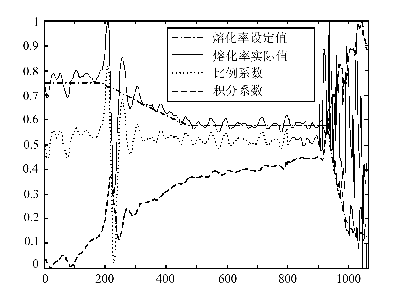
\includegraphics[width=6cm]{Image/01.eps}}
        \vskip 1mm{\small
            图1\quad 熔化率与比例、积分系数之间的关
            \\
            Fig.\,1\quad Comparing melting rate with proportion and integral parameters of the Consarc controller }
      }
    }
  \end{center}






  \TeX 的参考文献的引用比较方便,比如我们想引用Knuth的The \TeX
  book,可以输入``The \TeX book\verb|$^{[1]}$|''得到想要的效果``The
  \TeX book$^{[1]}$''.再比如我们输入``\verb|多模态优化问题\,\!$^{[2]}$|''得到想要的效果``多模态优化问题\,\!$^{[2]}$''.

  \subsection{作者简介注意事项}

  文章末页需附作者中英文简介,简介不超过100字,包括作者姓名、职称、学习工作经历,以及研究方向.


  作者照片请选用简单背景的证件照片,比例要求是$5:4$,大小做成3.0\,cm\,$\times$\,2.4\,cm.

  在无照片情况下,采用biographynophoto环境来填写作者简历.
  与正常情况的区别是,此时没有了照片文件这个参数.

  \section{其他注意事项}

  1) 因本刊文章为国内外公开发表,所有录用后稿件必须在本单位经保密审查.
  修改加工后的定稿除根据录用通知要求发送一份至编辑部指定电子邮箱外,
  另请一式两份,注明原稿件编号后附本单位同意公开发表的介绍信寄至编辑部.
  如无特殊原因,录用通知发出半年后才收到的修改稿,本刊不再发表.

  2)
  请作者仔细地按照录用通知和该模版中的各项要求认真加工修改稿,若修改稿不符合要求,编辑部将退回作者重新修改直至合乎要求为止,
  由此造成的稿件不能及时发表的责任由作者自负.
  作者如无特殊声明,本刊默认第一作者为通信作者.
  如果第一作者非文章通信作者或通信作者联系方式变动,
  务请及时通知编辑部.


\end{multicols}%开始通栏显示
\vskip1mm
\hrule
\begin{equation}
  T_{N-i}(m_{N-i})= \left[ \underbrace{O,\cdots,
    O}_{Z_1^{N-i}(m_{N-i})} \underbrace{I \cdot h^{N-i}(n^{N-i}), I
    \cdot h^{N-i}(n^{N-i}-1),\cdots, I \cdot
    h^{N-i}(m^{N-i})}_{L^{(N-i)}},\underbrace{O,\cdots,
    O}_{Z_2^{N-i}(m_{N-i})} \right]\tag{3}
\end{equation}
\begin{equation} \left[
    \begin{array}{c}
      \hat{{\pmb x}}(k+1) \\
      {\pmb e}(k+1)       \\
    \end{array}
    \right]=\left[
    \begin{array}{cc}
      A_0+B_0F+L_o(C(k)-C_0)               & L_oC(k)      \\
      (A(k)-A_0)+(B(k)-B_0)F-L_o(C(k)-C_0) & A(k)-L_oC(k) \\
    \end{array}
    \right]\left[
    \begin{array}{c}
      \hat{{\pmb x}}(k) \\
      {\pmb e} (k)      \\
    \end{array}
    \right]\tag{4}
\end{equation}
\begin{multicols}{2}%开始双栏显示

\end{multicols}%开始通栏显示

\begin{center}
  \vbox{\centering{\small 表1\quad 这是一个通栏的表格示例
      \\
      Table 1 \quad An exampletable in one column } \vskip2mm
    \renewcommand{\baselinestretch}{1.2}
    {\footnotesize\centerline{\tabcolsep=15pt\begin{tabular*}{\textwidth}{ccccc}
          \toprule
          对手 (OPP)                   & 比分 (CSU : OPP) & 团队决策所占比例 & 个体决策所占比例 & 团队决策与个体决策比值 \\
          \hline
          Cyberoos2001                &       3:0     &       71.5       &       28.5       &          2.51          \\
          FCPortugal2001              &       1:0     &       68.4       &       31.6       &          2.16          \\
          Gemini                      &      26:0     &       59.7       &       40.3       &          1.48          \\
          Harmony                     &       3:0     &       69.9       &       30.1       &          2.32          \\
          Lazarus                     &      11:0     &       57.3       &       42.7       &          1.34          \\
          MRB                         &       2:0     &       63.2       &       32.8       &          1.93          \\
          SBCe                        &       4:1     &       65.8       &       34.2       &          1.92          \\
          UvA\_Trilearn\_2001         &       1:0     &       54.9       &       44.1       &          1.24          \\
          UTUtd                       &      10:0     &       70.7       &       29.3       &          2.41          \\
          WrightEagle2001             &       3:1     &       66.2       &       33.8       &          1.96          \\
          Average                     &               &       64.8       &       35.2       &          1.84          \\
          \bottomrule
        \end{tabular*}}}}\end{center}

\begin{multicols}{2}%开始双栏显示
  \begin{center}
    {\centerline{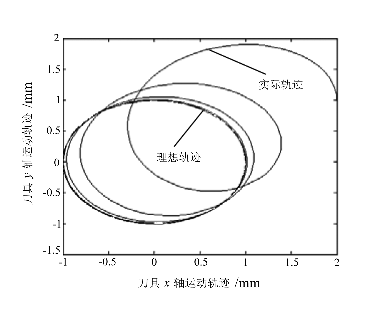
\includegraphics[width=6cm]{Image/02a.eps}}
      {\footnotesize (a)控制参数1\\(a) Controller parameter 1}} \\
    {\centerline{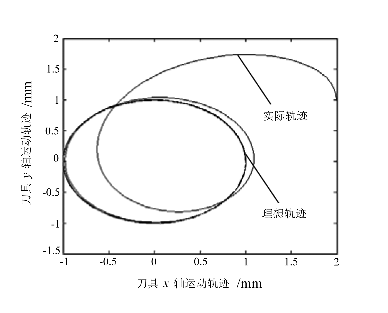
\includegraphics[width=6cm]{Image/02b.eps}} {\footnotesize
      (b)控制参数2\\(b) Controller parameter 2}} \vskip1mm {\small
      图2\quad 控制器参数对刀具运动轨迹的影响
      \\Fig.\,2\quad The influences
      of the controller parameters on the tracking errors}
  \end{center}

  3)
  稿件经编辑加工和排版后,编辑部将把pdf校样通过E-mail发送给通信作者,请务必逐字逐句核对并在三天内返回校样.
  除编辑和排版错误外请勿对校样内容作进一步的修改.
  校样内容的修改将导致因需要请同行专家对稿件作进一步评议而延误文章发表,因此而导致的后果和发生的费用将由作者承担.

  4) 在修改稿加工格式方面若有其他不明事宜,请来函来电垂询. 感谢合作!

  \section{结论}

  文章的结论请勿与摘要、前言等重复.

  \section*{致谢}

  文章作者可以在此处对支持和帮助其研究工作或本文写作的其他组织或人员表示感谢.
  注意,支持此研究的基金项目请直接标注在首页页脚处,不用在此再次致谢.

  \begin{thebibliography}{99}
    \zihao{6} \addtolength{\itemsep}{0.2em} \urlstyle{rm}
    \bibitem{bartkowiak2011anomaly} Bartkowiak, Anna M. Anomaly, novelty, one-class classification: a comprehensive introduction. {\sl Robotics and Autonomous Systems}, 2011, {\bf 44}(3): 61$-$71


    \bibitem{1} Ran B, Boyce D E. {\sl Modeling Dynamic Transportation Network}.
    Berlin: Springer-Verlag, 1996. 69$-$83

    \bibitem{2} Payton D, Estkowski R, Howard M. Compound behaviors in pheromone robotics. {\sl Robotics and Autonomous Systems}, 2003, {\bf 44}(3): 229$-$240

    \bibitem{3} Su Lian-Cheng, Zhu Feng. Design of a novel omnidirectional stereo vision system. {\sl  Acta Automatica Sinica}, 2006,{\bf 32}(1): 67$-$72\\ (苏连成, 朱枫. 一种新的全向立体视觉系统的设计. 自动化学报, 2006, {\bf 32}(1): 62$-$72)

    \bibitem{4} Roychoudhury R, Bandyopadhyay S, Paul K. Adistributed mechanism for topology discovery in ad hoc wireless networks using mobile agents. In: Proceedings of IEEE First Annual Workshop on Mobile and Ad hoc Networking and Computing. NewYork, USA: IEEE, 2000. 145$-$146
    \bibitem{5} Hryniewicz O. An evaluation of the reliability of complex systems using shadowed sets and fuzzy lifetime data. {\sl International Journal of Automation and Computing}, to be published

    \bibitem{6} Zhang W. Reinforcement Learning for Job-Shop Scheduling [Ph.\,D.
        dissertation], Peking University, 1996

    \bibitem{7} The Math Works.Image Processing Toolbox for Use with Matlab: User$'$s Guide [Online], available: http://www.mathworks.com, November 3, 2006

    \bibitem{8} Reily R C, Mack J L. The Self-organization of Spatially Invariant
    Representations, Technical Report PDP.CNS.92.5, Department of
    Psychology, Mellon University, USA, 1993

    \bibitem{9} Wilkinson J P. Nonlinear Resonant Circuit, U.\,S. Patent 362412, July 1990

    \bibitem{10} IEEE Criteria for Class IE Electric System, IEEE Standard 308, 1969

    \bibitem{11} IEEE Criteria for Class IE Electric System, IEEE Standard 308, 1969
    \bibitem{12} IEEE Criteria for Class IE Electric System, IEEE Standard 308, 1969
  \end{thebibliography}

  \begin{biography}[Image/ssl.eps]
    \noindent{\hei
      尚书林
    }\quad
    中国科学院自动化研究所博士研究生.
    2002年获得北京师范大学信息学院电子系学士学位.
    主要研究方向为图像与视频压缩技术.\\E-mail: aas\_editor@ia.ac.cn

    \noindent({\bf
      SHANG Shu-Lin
    }\quad
    Ph.\,D. candidate at the
    Institute of Automation, Chinese Academy of Sciences. He received
    his bachelor degree from Beijing Normal University in 2002. His research
    interest covers image compression and video coding.)
  \end{biography}

  \begin{biography}[Image/nmzuo.eps]
    \noindent{\hei
      左年明
    }\quad
    中国科学院自动化研究所博士研究生.
    2002年获得山东大学数学学院学士学位.
    主要研究方向为医学图像处理, CT图像重建.\\E-mail: aas\_editor@ia.ac.cn

    \noindent({\bf
      ZUO Nian-Ming
    }\quad
    Ph.\,D. candidate at the
    Institute of Automation, Chinese Academy of Sciences. He received
    his bachelor degree from Shandong University in 2002. His research
    interest covers medical CT image reconstruction and medical image
    processing.)
  \end{biography}

  \begin{biographynophoto}
    \noindent{\hei 陈培颖}\quad 《国际自动化与计算杂志》编辑部责任编辑.\\E-mail: peiying.chen@ia.ac.cn

    \noindent({\bf CHEN Pei-Ying}\quad Managing editor at the Editorial Office of
    {\sl International Journal of Automation and Computing}.)
  \end{biographynophoto}

  \begin{biographynophoto}
    \noindent{\hei 欧\hskip2.5mm彦}\quad 《自动化学报(英文版)》编辑部责任编辑.\\E-mail: yan.ou@ia.ac.cn

    \noindent({\bf OU Yan}\quad Managing editor at the Editorial Office of
      {\sl IEEE/CAA Journal of Automatica Sinica (JAS)}.)
  \end{biographynophoto}

  \begin{biography}[Image/zz.eps]
    \noindent{\hei
      张\hskip2.5mm哲
    }\quad
    《国际自动化与计算杂志》与《自动化学报》编辑部技术编辑. 2006年获得北京工业大学电控学院自动化系学士学位.
    本文通信作者.\\E-mail: zhe.zhang@ia.ac.cn

    \noindent({\bf
      ZHANG Zhe
    }\quad
    Copy-editor at the Editorial Office of
    {\sl International Journal of Automation and Computing}, and {\sl
      Acta Automatica Sinica}. He received his bachelor degree from Beijing
    University of Technology in 2006. Corresponding author of this paper.)
  \end{biography}
\end{multicols}
\end{document}
